% -*- root: haynes-notes.tex -*-

\section{The stable category} % <<<
\label{TheStableCategory}
\ifx\OutputTheStableCategory\undefined\else
In order to set up the spectral sequence alluded to above, whose $E^1$ page consists of the stable homotopy groups of spheres in each column, it's a good idea to talk about stable homotopy a bit; for more information, see Adams' blue book~\cite{Adams}.  The notation $[X, Y]$ will mean pointed homotopy classes of point maps.  There is a map $\Suspend: [X, Y] \to [\Suspend X, \Suspend Y]$, and the idea is to study this game in detail.\todo{``game''?}

One nice thing about suspending is that when you suspend you get a group: $[\Suspend X, Z]$ is a group naturally in $X$ and $Z$, and $[\Suspend^2 X, Z]$ is abelian.  The group structure comes from
\begin{ctikzcd}[column sep = 2.7em]
(g_1 + g_2): \Suspend X \rar["\textup{pinch}"] &  \Suspend X \wsum \Suspend X \rar["g_1 \wsum g_2"] &  Z \wsum Z \rar["\textup{fold}"] & Z
\end{ctikzcd}
``Naturally in $Z$'', for example, means that given $f: Z \to Y$, in
\begin{ctikzcd}
\Suspend X \rar["g_1",yshift=0.3em] \rar["g_2"',yshift=-0.3em] & Z \rar{f} & Y
\end{ctikzcd}
we have $f_*(g_1 + g_2) = f_* (g_1) + f_* (g_2)$ in $[\Suspend X, Y]$. This holds because the fold map is a natural transformation from $X\mapsto X\vee X$ to the identity functor, and so the following diagram commutes:
\begin{ctikzcd}[column sep = 2.7em]
&&&[-1/2\pgfmatrixcolumnsep]Y\vee Y\drar["\textup{fold}"anchor=south, sloped]&[-1/2\pgfmatrixcolumnsep]\\
%
\Suspend X \rar["\textup{pinch}"]\ar[drrr,"g_1+g_2"'anchor=north, sloped, yshift=-0.1em ] &
\Suspend X\vee \Suspend X \rar["g_1\vee g_2"]\ar[urr,start anchor={[yshift=0.1em]north east},end anchor= west,"(fg_1)\vee (fg_2)"anchor=south,sloped]  &
Z\vee Z \urar["f\vee f"{anchor=south,xshift=-0.4em}, sloped]\drar["\textup{fold}"anchor=south, sloped]
&& Y\\
%
&&&Z\urar["f"]
\end{ctikzcd}
The top path is the map $f_*(g_1)+f_*(g_2)$ and the bottom, the map $f_*(g_1+g_2)$.

Note, however, that the group structure on $[\Suspend X, Z]$ is not natural in $\Suspend X$.
As an example, consider the Whitehead square\footnote{Essentially, we are showing that the \emph{map} $w_n$ is not in the image of the suspension map $[S^{2n-2}, S^{n-1}] \to [S^{2n-1}, S^n].$}
\begin{ctikzcd}
S^{2n-1} \rar{w_n}& S^n.
\end{ctikzcd}
The induced function $w_n^* = [S^n, S^n] \to [S^{2n-1}, S^n]$ is not a homomorphism for $n$ even.  To see this, recall that $w_n = [\iota_n, \iota_n] \in \pi_{2n-1} (S^n)$ is defined by
\begin{ctikzcd}
S^{2n-1} \drar["W"']\rar{w_n} & S^n \\
& S^n \wsum S^n\uar["\textup{fold}"'],
\end{ctikzcd}
where $W$ is the attaching map for $S^{2n-1} \xrightarrow{W} S^n \wsum S^n \to S^n \times S^n=C(W)$. The following diagram commutes, by definition of $2 \iota_n$:
\begin{ctikzcd}[column sep=large]
S^{2n-1} \drar["W"']\rar{w_n} & S^n  \rar["2\iota_n"]& S^n \\
& S^n \wsum S^n\uar["\textup{fold}"']\rar["2\iota_n\wsum2\iota_n"]& S^n \wsum S^n\uar["\textup{fold}"'],
\end{ctikzcd}

The top row represents $(\iota_n + \iota_n) \circ w_n = w_n^*(2 \iota_n)$, the lower composite represents $[2\iota_n, 2\iota_n] = 4[\iota_n, \iota_n]$ (by bilinearity of the Whitehead product), which is equal to $4 w_n$ or $4 w_n^*(\iota_n)$, and the diagram is a witness to \[w_n^*(2 \iota_n) = 4 w_n^* \iota_n.\]  So $w_n^*$ cannot be a homomorphism unless $w_n = w_n^* \iota_n$ has finite order in $\pi_{2n-1}(S^n)$.  But for $n$ even, $h(w_n) = 2 \iota_n$, so the image of $w_n$ under the Hopf map is infinite cyclic!

The way to get around the presence of non-homomorphic maps is by suspending more.  In what follows we take $X$ and $Y$ to be finite complexes.  Then we define $\{X, Y\} = [\Suspend^n X, \Suspend^n Y]$ for $n$ much larger than 0. In particular, the following theorem shows that for $n$ sufficiently large $[\Suspend^n X, \Suspend^n Y] \cong [\Suspend^{n+1} X, \Suspend^{n+1} Y]$, and we define $\{X, Y\}$ to be this ``stable'' group, the ``stable homotopy classes of maps'' between $X$ and $Y$.
\begin{thm}[Freudenthal suspension theorem]
If $Y$ is an $(n-1)$-connected CW-complex, and $X$ is a finite dimensional CW-complex of dimension $d$, then $\Sigma:[X,Y]\to[\Sigma X,\Sigma Y]$ is surjective when $d\leq2n-1$ and an isomorphism when $d<2n-1$.
\end{thm}
Now composition gives a product
\begin{ctikzcd}
\{X, Y\} \times \{Y, Z\} \rar & \{X, Z\}
\end{ctikzcd}
which is bilinear since we can assume all maps involved are in the image of $\Suspend$.

So we get a category whose objects are finite complexes and whose morphisms are stable homotopy classes of pointed maps.  Some important properties of this category are:
\begin{enumerate}
\item We've just seen that the category is pre-additive.
\item It has coproducts: if $X$ and $Y$ are finite complexes, $X \wsum Y$ is the coproduct in this category: \[\{X \wsum Y, Z\} = \{X, Z\} \times \{Y, Z\}.\]  This is true because of the homotopy equivalence $\Suspend^n(X \wsum Y) \simeq \Suspend^n X \wsum \Suspend^n Y$.
\item Well, these two facts together mean that now $X \wsum Y$ is the \emph{product} on our category as well!  Using the collapse maps out of $X \wsum Y$ to $X$ and $Y$, we have to show that $\{W, X \wsum Y\} \to \{W, X\} \times \{W, Y\}$ is an isomorphism.
\begin{enumerate}
\item Surjectivity.  If $f: \Suspend^n W \to \Suspend^n X$ and $g: \Suspend^n W \to \Suspend^n Y$ represent an element of $\{W, X\} \times \{W, Y\}$, then $\Suspend^n W \to \Suspend^n W \wsum \Suspend^n W  \xrightarrow{f \wsum g} \Suspend^n X \wsum \Suspend^n Y$ pushes forward to $(f, g)$.
\item Injectivity. Suppose that $f\in\{W,X\vee Y\}$ maps to zero under the above map. Then noting that $[\Suspend^n W, \Suspend^n X] \times [\Suspend^n W, \Suspend^n Y] \cong [\Suspend^n W, \Suspend^n X \times \Suspend^n Y$], the composite $kf$ is null:
\begin{ctikzcd}
\Suspend^n W\ar[r]{f} & \Suspend^n X \wsum \Suspend^n Y\ar[r]{k} & \Suspend^n X \times \Suspend^n Y
\end{ctikzcd}
%\begin{diagram}[height=2em]
%\Suspend^n W & \rTo_f & \Suspend^n X \wsum \Suspend^n Y \\
%\dInto & \ruDashto & \dTo_k \\
%C \Suspend^n W & \rTo^H & \Suspend^n X \times \Suspend^n Y
%\end{diagram}
%To show that $f$ is stably null, we have to lift $H$ to the dashed arrow, by taking $n$ large enough.
In particular, $f$ lifts to the fiber $F(k)$. Now the fiber is $(2n-1)$-connected, so when $n > \dim W$, the lifting must be null,\footnote{Recall that by CW-approximation, a $(2n-1)$-connected CW-complex is homotopic to a complex with no nonzero cells of dimension less than $2n$. By CW-approximation, all maps $C(\Sigma^n W)\to \Sigma^nX\vee\Sigma^n Y$ will be null when $n>\dim W$.} and we're done.
\end{enumerate}
\end{enumerate}

So the wedge is the product in this category.  Now let's add ``formal desuspensions.''  The point is that now that $\Sigma:\{X, Y\}\to\{\Suspend X, \Suspend Y\}$ is an isomorphism, we've really obliterated the difference between the morphism sets here, and $\Suspend$ has become a fully faithful functor.  Now we'll make it into an isomorphism.  To fix it up, we'll simply put in formal desuspensions.

The new category, the $S$-category, has as objects pairs $(X, n)$, where $X$ is a finite complex and $n$ is an integer, the ``formal $n$-fold suspension of $X$.''  And $\Hom\{(X, m), (Y, n)\} = [\Suspend^{m+k} X, \Suspend^{n+k} Y]$ for $k$ much larger than 0, namely $k$ big enough that $ m+k\geq0$, $n+k\geq0$, and larger still so that one is in the stable range.

Note that $(X, 1) \xrightarrow{\cong} (\Suspend X, 0)$, i.e., the ``formal suspension'' is isomorphic to the informal suspension.  So we write $(X, n)$ and $\Suspend^n X$ and $\Hom\{(X, m), (Y, n)\}$ as $\{\Suspend^m X, \Suspend^n Y\}$.  But now we have the object $(X, -1) = \Suspend^{-1} X$.  And so we talk about objects like $\{S^0, S^{-1}\}=[S^k, S^{k-1}]$ for $k$ sufficiently large, which we know to be $\Zbb_2$.

As an example of how things work, remember earlier we studied the group $J(X)$ which had to do with stable fiber homotopy equivalence.  Let $V\downarrow X$ be an $(n-1)$-sphere bundle.  In lecture \ref{FactsAboutThomSpaces}, we saw that if $V\downarrow X$ is fiber homotopy trivial, there is a splitting
\begin{ctikzcd}
T(V) \rar & S^n \\
S^n\uar\urar["\simeq"].
\end{ctikzcd}
Also we found out that such a coreduction meant that $S^0 \ast_X V \to X$ is fiber-homotopy trivial.\footnote{$S^0 \ast_X V \to X$
is the fiberwise suspension of $V$. If $V$ is the sphere bundle of a vector bundle, fiberwise suspension corresponds to adding a trivial bundle.
}
And so now in our new category we find
\begin{lem}
$V\downarrow X$ is stable fiber homotopy trivial if and only if $S^n \to T(V)$ has a stable retraction.
\end{lem}
In the $S$-category, the left--hand condition is $T(V) \simeq \Suspend^n (\Xpt)$ and the right--hand condition is that $T(V) \simeq S^n \wsum (\mathrm{something})$, and these agree.

Now earlier we also sketched a proof of Atiyah that $\widetilde J(X)$ is finite over a finite complex; so for any $V\downarrow X$ there is an $n$ so $V^{\ast n}\downarrow X$ is stably fiber homotopy trivial.  So that says that in the $S$-category, $\{T(V^{\ast k})\}$ is periodic up to suspension.  This is ``James periodicity.''

As a final remark, note that now we can talk about the Thom space of certain virtual bundles: \[T(V - \varepsilon_n) = \Suspend^{-n} T(V).\]

% >>>
\fi
\BoxedNote{}







\section{Homotopical algebra and duality} % <<<
\label{HomotopicalAlgebraAndDuality}
\ifx\OutputHomotopicalAlgebraAndDuality\undefined\else
Well, let's continue with the discussion of stable homotopy, and really enter the stratosphere at this point, at least for a short while.  So remember last time we ended with the notion of a category $\Ccat$, the $S$-category of finite complexes.  In this category there is an important notion of ``exact triangles'': $X \to Y \to Z \to \Suspend X$ is an exact triangle if it is homotopy equivalent to $X \xrightarrow{f} Y \to Cf \to \Suspend X$ on the level of spaces, perhaps after suspending a lot.  Two important facts about exact triangles are
\begin{enumerate}
\item A sequence $X \to Y \to Z \to \Suspend X$ is exact iff it remains exact after application of $\{W, -\}$ for all $W \in \Ccat$.\todo{We should be careful and distinguish function spaces from the set of stable homotopy classes.}
\item $Y \xrightarrow{g} Z \to \Suspend X \xrightarrow{\Suspend f} \Suspend Y$ is an exact triangle iff $X \xrightarrow{f} Y \xrightarrow{g} Z \to \Suspend X$ is an exact triangle.
\end{enumerate}
This is somehow reminiscent of (co)homology. To make that hint precise, consider a category $\Scat$, the ``stable category of spectra'', with the following properties:
\begin{itemize}
\item It contains the category $\Ccat$.
\item $\Scat$ has exact triangles, and the inclusion of $\Ccat$ into $\Scat$ takes exact triangles to exact triangles.
\item $\Scat$ is additive: it has products $\prod$ and coproducts $\coprod$, and finite products and finite coproducts coincide.
\item The equivalence $\Suspend$ on $\Ccat$ extends to one on $\Scat$.
\item $\Scat$ has smash products with nice properties, e.g.: $W \sprod: \Scat \to \Scat$ preserves exact triangles; $S^0 \sprod$ is a unit.
\item ``Brown representability'' holds.
\item ``Whitehead representability'' holds.
\end{itemize}

What do these last two mean?  They have to do with cohomology and homology, so we'd better know what those are: a function $E^0: \Scat^{op} \to \Ab$ is cohomological if
\begin{enumerate}
\item $E^0$ sends exact triangles to exact sequences.
\item $\Scat$ is going to contain infinite complexes, so we'd better know what $E^0$ does to colimits, e.g., wedges. It must satisfy the ``Milnor axiom'', that the following natural map is an isomorphism:
\[
E^0\left({\bigvee}_\alpha X_\alpha\right) \xrightarrow{\cong} \prod_\alpha E^0 X_\alpha
.\]
\end{enumerate}
If $E^0$ is cohomological, we define $E^q (X) := E^0 (\Suspend^{-q} X)$. ``Brown representability'' states that any cohomological functor (a.k.a.\ cohomology theory) of $\Scat$ is representable: there is a spectrum $E$ such that the functors $E^0$ and $\{\textup{---}, E\}$ are naturally isomorphic.\footnote{Note that in this context, the restriction of $E^0$ to spaces always refers to \emph{reduced} $E$-cohomology, so usually the twiddle is left out.}  Analogously, $E_0: \Scat \to \Ab$ is homological if
\begin{enumerate}
\item $E_0$ sends exact triangles to exact sequences, and
\item The Milnor axiom holds: the natural map $\bigoplus_\alpha E_0 X_\alpha \xrightarrow{\cong} E_0(\bigvee_\alpha X_\alpha)$ is an isomorphism.
\end{enumerate}
Whitehead representability says any homology theory is representable: there is a spectrum $E$ so that $E_0$ is naturally isomorphic to the functor $\{S^0, \text{---} \sprod E\} \cong \pi^S_0(\text{---} \sprod E)$.  If you look at Adams' blue book~\cite{Adams}, you'll see how to construct $\Scat$, with lots of technical details.  For now, we'll just see what an object, i.e., a spectrum, is.  One construction takes a spectrum to be a sequence $\ldots, E_{n-1}, E_n, E_{n+1}, \ldots$ of pointed spaces, with pointed maps $\Suspend E_n \to E_{n+1}$.  Two examples:
\begin{enumerate}
\item Take $X$ a pointed space, define a spectrum $\SuspendS X$ by \[(\SuspendS X)_n =\begin{cases} \Suspend^n X,&n\geq0\\\ptspace,&n<0.\end{cases}\]
This gives a name to the inclusion functor from the homotopy category of pointed spaces to $\Scat$, which has an adjoint function $\LoopsS$ that goes the other way.  in particular, there are maps
\begin{ctikzcd}
X \rar{\alpha} & \LoopsS \SuspendS X, \\
E & \lar["\beta"'] \SuspendS \LoopsS E.
\end{ctikzcd}
\item Fix an abelian group $A$; define the spectrum $HA$
\[(HA)_n =\begin{cases} K(A,n),&n\geq0\\\ptspace,&n<0.\end{cases}\]
The map $\Suspend K(A, n) \to K(A, n+1)$ is given by the adjoint of the identity $K(A, n) \to \Loops K(A, n+1)$.
\end{enumerate}

Now let's talk about a notion of duality that makes sense in the context of spectra.  This is where we lift off a bit; Michael Artin says this is the hardest thing in the world to write down.  A duality is a map $\alpha: X \sprod Y \to S^0$ such that for all $W \in \Scat$, the composite \[\{W, Y\} \xrightarrow{X \sprod} \{X \sprod W, X \sprod Y\} \xrightarrow{\alpha_*} \{X \sprod W, S^0\}\] is an isomorphism. In other words, given a map $f: W \to Y$, we can form the composite:
\[X\wedge W \xrightarrow{1_X \wedge f} X\wedge Y\to S^0,\]
and we require that this assignment on Hom-sets is an isomorphism.
\todo{Address this ConfusedBox.}
\ConfusedBox{Do we need another axiom here? I once saw:

A map $u:S\to A\wedge A^\perp$ is called a duality if for all $E$, the maps
%\[[A,E]\to[S,E\wedge A^\perp],\qquad (A\to E)\mapsto (S\to A\wedge A^\perp\to
\begin{alignat*}{2}
u_E:[A,E]\to[S,E\wedge A^\perp],&\qquad &
(A\to E)\mapsto (S\to A\wedge A^\perp\to E\wedge A^\perp)\\
u^E:[A^\perp,E]\to[S,A\wedge E],&\qquad &
(A^\perp\to E)\mapsto (S\to A\wedge A^\perp\to A\wedge E)
\end{alignat*}
are isomorphisms. Duality is symmetric, as smash product is homotopy
commutative. Moreover, given two dualities, we have isomorphisms
$[A,B]\longrightarrow[S,B\wedge A^\perp]\longleftarrow[B^\perp,A^\perp]$, so
that we can define the adjoint $f^\perp:B^\perp\to A^\perp$ of a map $f:A\to B$.}

The first thing to note is that these dualities exist:
\begin{thm}
For all $X$ there is a $Y$ with a duality $X \sprod Y \to S^0$.
\end{thm}
\begin{proof}
$W \mapsto \{X \sprod W, S^0\}$ is a cohomology theory, so it has a representing spectrum $Y$; hence there is a natural isomorphism $\{X \sprod W, S^0\} \cong \{W, Y\}$.  The map $\alpha$ comes from taking for $W$ the spectrum $Y$ itself: $\{X \sprod Y, S^0\} \cong \{Y, Y\}$.  Let $\alpha$ be the element of $\{X \sprod Y, S^0\}$ corresponding to the identity.  The naturality of Brown representability gives us that the isomorphism comes in the manner described in the definition of duality: for any $W \in \Scat$, $\gamma \in \{W, Y\}$:
\begin{ctikzcd}
|[xshift=-2em]|\gamma \ar[r,mapsto] & \id\sprod \gamma \rar[mapsto] & ? \ar[r,mapsto] &|[xshift=2em]| \gamma\\[-1em]
%%
 \{W, Y\} \rar{X \sprod} & \{X \sprod W, X \sprod Y\} \rar{\alpha_*} & \{X \sprod W, S^0\} \rar["BR", "\cong"'] & \{W, Y\} \\
 \{Y, Y\} \rar{X \sprod}\uar["\gamma^*"'] & \{X \sprod Y, X \sprod Y\} \rar{\alpha_*} \uar["\gamma^*"'] & \{X \sprod Y, S^0\} \uar["\gamma^*"']\rar["BR", "\cong"'] & \{Y, Y\} \uar["\gamma^*"'] \\[-1em]
%%
|[xshift=-2em]|\id\ar[uuu,mapsto,bend left=15]\ar[mapsto,r] & \id\rar[mapsto]& \alpha\ar[r,mapsto] &|[xshift=2em]| \id\ar[uuu,mapsto,bend right=15]
\end{ctikzcd}


The first two squares obviously commute; the third commutes by naturality of Brown representability.
\end{proof}

In fact there's more to be had from this use of Brown representability: the correspondence $X \leadsto Y = DX$ can be made into a contravariant functor in such a way that $X \sprod DX \xrightarrow{\alpha_X} S^0$ is a natural transformation.  That is, we can construct a functor $D:\Scat^\text{op}\to\Scat$ and a natural collection $\alpha_X:X\wedge D(X)\to S^0$ for $X\in\Scat$ of dualities. By ``natural'', we mean that for any map\todo{Put a footnote explaining this dinaturality or whatever it's called.} %\IncorrectFootnote{$\alpha$ is a natural transformation of functors $\Scat\times\Scat^\text{op}\to\Scat$, where $S^0$ is the functor whose image is the object $S^0$ and its identity morphism.} For
$f: X \to Y$, the following diagram commutes:
\begin{ctikzcd}
X \sprod DY\dar["f\sprod 1"'] \rar{1 \sprod Df} & X \sprod DX\dar["\alpha_X"] \\
Y \sprod DY \rar{\alpha_Y} & S^0
\end{ctikzcd}
To make the dualities this way, we first use the axiom of choice to pick a dual $DX$ for each object $X$, and we obtain maps $\alpha_X$ in the manner described above.  Now for any map $f: X \to Y$ we get, for any $W \in \Scat$, a map $\gamma$ via
\begin{ctikzcd}
\{W, DY\}\dar[equal,"BR"] \rar{\gamma} & \{W, DX\}\dar[equal,"BR"] \\
\{Y \sprod W, S^0\} \rar{(f \sprod 1)^*} & \{X \sprod W, S^0\}.
\end{ctikzcd}
Take $W = DY$, then define $Df: \{DY, DY\} \to \{DY, DX\}$ by $1 \mapsto Df$.  Then we have
\begin{ctikzcd}
Df \rar[mapsto] & 1 \sprod Df \rar[mapsto] & \alpha_X \circ (1 \sprod Df) \rar[mapsto]  & |[xshift=2.5em]|Df \\[-1em]
%%
\{DY, DX\} \rar{X \sprod} & \{X \sprod DY, X \sprod DY\} \rar{\alpha_{X*}} & \{X \sprod DY, S^0\} \rar["BR", "\cong"'] & \{DY, DX\} \\
\{DY, DY\} \rar{Y \sprod} & \{Y \sprod DY, Y \sprod DY\} \rar{\alpha_{Y*}} & \{Y \sprod DY, S^0\} \uar["(f\sprod1)^*"']\rar["BR", "\cong"'] & \{DY, DY\} \uar["\gamma"']\\[-1em]
%%
\id \rar[mapsto] & \id \rar[mapsto] & \alpha_Y \rar[mapsto] & |[xshift=2.5em]| 1\ar[uuu,mapsto,bend right=15],
\end{ctikzcd}
where the vertical map sends $\alpha_Y$ to $\alpha_Y \circ (f \sprod 1)$.  The maps in the rows are determined by the construction of the dualities involved; the last square commutes by definition of $Df$, and the two composites at $\{X \sprod DY, S^0\}$, which are equal, are the two ways of going around the square that we wanted to show commutes.

All right, enough, let's see what having $D$ does for us.
\begin{lem}
\begin{itemize}
\item We can choose $DS^0 = S^0$.
\item $D \Suspend X = \Suspend^{-1} D X$.
\item $X \to Y \to Z \to \Suspend X$ an exact triangle means that $DX \from DY \from DZ \from \Suspend^{-1} DX$ is an exact triangle.
\end{itemize}
\end{lem}
\begin{cor}
A finite complex is built out of spheres using exact triangles, so we get
\begin{itemize}
\item $D$ of a finite spectrum is finite.
\item If $K$ is finite, then $D(K \sprod X) \simeq DK \sprod DX$ (but not if $K$ is infinite; in general $D$ isn't nice when there are limits around).
\item If $K$ is finite, then $K$ can be taken for $DDK$.
\end{itemize}
\end{cor}
\ConfusedBox{The whole function spectrum spiel had been omitted, I took the following remark from the end of the next chapter, where it had been misplaced.}
\begin{rem}
The defining property of $D$ was $\{W, DX\} \cong \{X \sprod W, S^0\}$.  Now there's nothing particularly special about $S^0$: if $Y$ is any spectrum, $W \mapsto \{X \sprod W, Y\}$ is a cohomology theory for $W$, so it's represented by a spectrum $F(X, Y)$.  If you think of $X \sprod W$ as a tensor product, $F(X, Y)$ is a like a hom-space.  So think of $F(X, Y)$ as a ``function spectrum,'' and $DX = F(X, S^0)$.  It doesn't come to us the way that function spaces normally do; we get it out of Brown representability.

Notice that there is a map $f: DX \sprod Y \to F(X, Y)$ defined by
\begin{ctikzcd}[column sep=tiny]
\{X \sprod (DX \sprod Y), Y\} \dar[equal]\ni &[-\columnsep-0.6em] (X \sprod DX \sprod Y \ar[rr,"\alpha_*\sprod1"]&\dar[mapsto]& S^0 \sprod Y \ar[r,"\id"]&[1em] Y) \\
\{DX \sprod Y, F(X, Y)\} & &f.
\end{ctikzcd}
\todo[noline]{Can we make this diagram suck less?}
Now we'd like $f$ to be an equivalence; this isn't always true, but given some reasonable condition, say $X$ or $Y$ a finite complex, then it is.
\end{rem}
% >>>
\fi
\BoxedNote{}






\section{Dualities} % <<<
\label{Dualities}
\ifx\OutputDualities\undefined\else
We were talking about duality; the last thing mentioned was the ``function spectrum'' $F(X, Y)$ satisfying $\{W, F(X, Y)\} \cong \{X \sprod W, Y\}$ for all $W \in \Scat$.  If $X$ is finite then $F(X, Y) = (DX) \sprod Y$.  Now call $Y = E$, take $W = S^n$, and assume $X$ is finite. Then,
\begin{ctikzcd}
\pi_n(DX\wedge E)\dar[equal]\rar[equal]&\{S^n,DX\wedge E\}\rar{\cong}&\{\Sigma^nX,E\}\dar[equal]\\
E_n(DX)\ar[rr,"\cong"',"\text{duality}"]&&E^{-n}(X)
\end{ctikzcd}
We want to relate this duality to other familiar dualities.  For example, how can we recognize a duality?  Suppose $X$ is finite and we have a map $\fhat: X \sprod Y \to S^0$; then $\fhat$ corresponds to a map $f: Y \to DX$ which makes the following triangle commute.
\begin{ctikzcd}
& X \sprod DX\dar["\alpha_X"] \\
X \sprod Y\urar["1\sprod f"]  \rar["\fhat"'] & S^0.
\end{ctikzcd}
 One could ask whether $f$ is an equivalence. Given a spectrum $E$ consider the following diagram:
\begin{ctikzcd}[column sep=-1.3em]
\mathclapph{E^{-n}(X)}{E_n(Y)} \ar[dd,"\fhat/"']\rar[equal] & \{S^n, Y\wedge E\} \dar\rar["(f\sprod 1_E)_*"] &[-\columnsep+5.5em] \{S^n,DX\sprod E\} \dar\rar[equal] & E_n(DX)\ar[dd,"\cong"]\\
& \{X\sprod S^n,X\sprod Y\sprod E\}\dar["(\fhat\sprod 1_E)_*"] \rar["(1_X\sprod f\sprod 1_E)_*"] & \{X\sprod S^n,X\sprod DX\sprod E\}\dar["(\alpha_X\sprod 1_E)_*"]\\
E^{-n}(X)\rar[equal] & \{X\sprod S^n,E\} \rar[equal] & \mathclapph{\{S^n,DX\sprod E\}}{\{X\sprod S^n,E\}}\rar[equal]& E^{-n}(X)
\end{ctikzcd}

In light of this diagram, if the obvious construction using $\fhat:X\wedge Y\to S^0$ actually produces an isomorphism $\fhat/$, then $f$ is an $E$-homology equivalence. That is, $f_*: E_n (Y) \to E_n (DX)$ is an isomorphism.

Note that if $X$ and $Y$ are finite spectra, and $f: X \to Y$ is an isomorphism on $H_*(-; \Zbb)$, then $f$ is an equivalence (there's no $\pi_1$ problem here).  So taking $E = H(-; \Zbb)$ will be enough.  That's what the standard duality theorems give you.

%\begin{wrapfigure}{r}{0.25\textwidth}
%\centering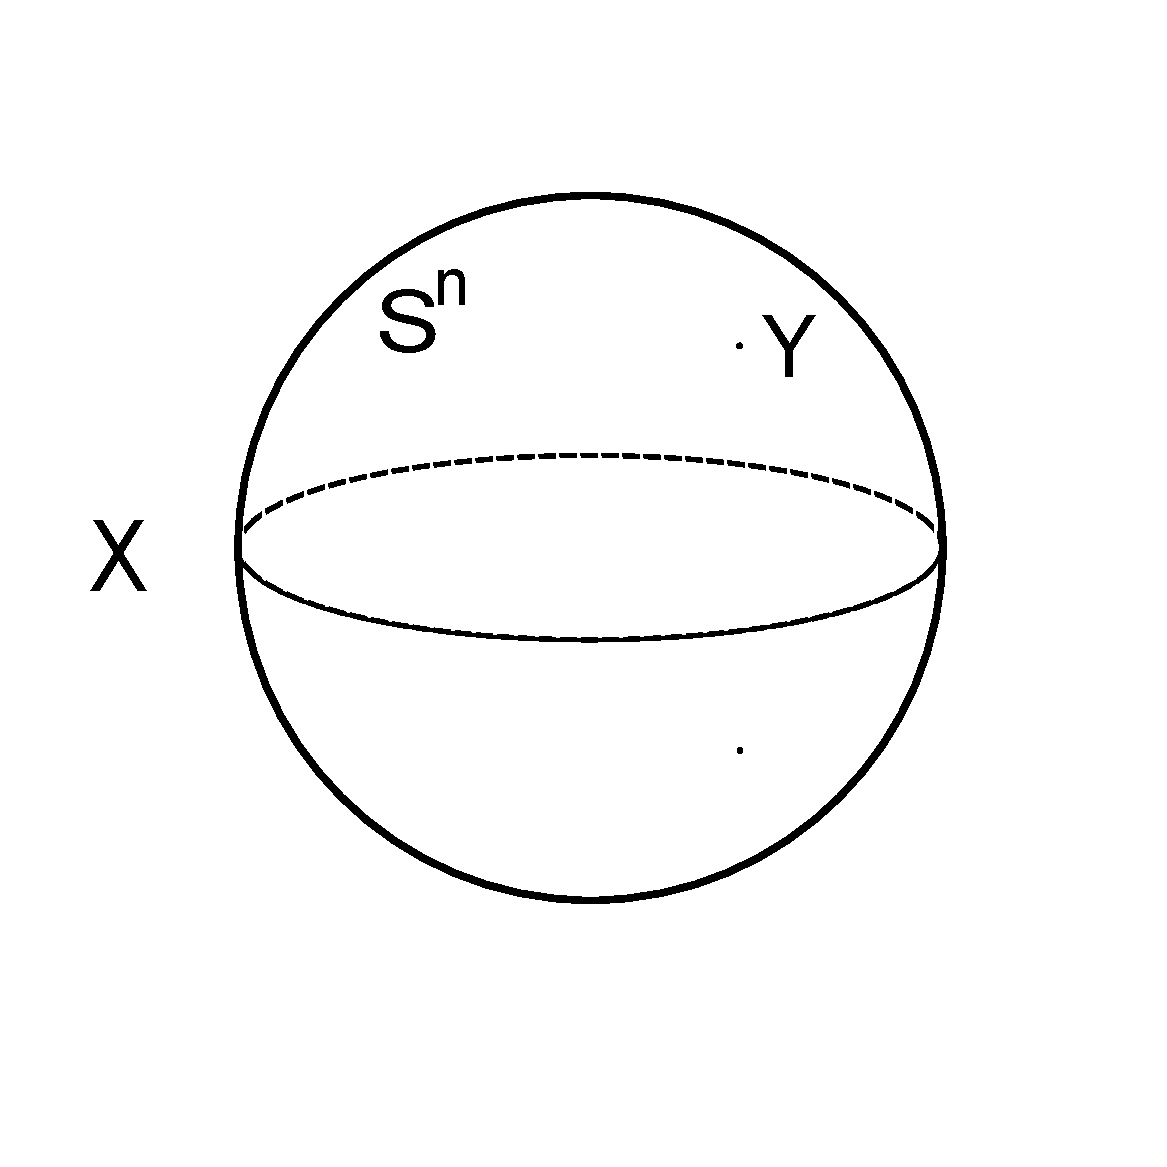
\includegraphics[width=0.2\textwidth]{figures/25.pdf}
%\caption{\small $X$ and $Y$ embedded in $S^n$.}
%\end{wrapfigure}
\subsection*{Alexander duality}
Let $X$ be a finite complex embedded in $S^n$; let $Y$ be another complex disjoint from $X$ in $S^k$. Fix a point $p$ not in $X$ or $Y$, and consider the stereographic projection $\textup{St}_p:S^n\setminus\{p\}\to\Rbb^n$.  Consider the map
\begin{cjointikzcd}
\diagram  X \times Y  \rar & S^{n-1}
%
\diagram \intertext{defined by}
%
\diagram (x, y)  \rar[mapsto] & \frac{\textup{St}_p(x)-\textup{St}_p(y)}{\|\textup{St}_p(x)-\textup{St}_p(y)\|}
\end{cjointikzcd}
%\begin{align*}
%X \times Y & \to S^{n-1} \\
%(x, y) & \mapsto \frac{x-y}{\|x-y\|}
%\end{align*}
and apply the Hopf construction to get a map
\begin{ctikzcd}
\Sigma(X\wedge Y)\rar["\simeq"] & X\ast Y \rar & S^n.
\end{ctikzcd}
In the category $\Scat$ we get a map $\fhat: X \sprod \Suspend^{1-n} Y \to S^0$.  Alexander duality says
\begin{thm}
If $Y \simeq S^n - X$ then $\fhat$ is a duality; $DX \simeq \Suspend^{1-n} Y$.
\end{thm}
\noindent The proof consists of showing that $\fhat/: \widetilde H_i (\Suspend^{1-n} Y) \xrightarrow{\cong} \widetilde H^i (X)$ is an isomorphism for $i \in \Zbb$.
\begin{rem}
If you think of $X$ and $Y$ as embedded in $\Rbb^n$ instead of $S^n$ and $Y \simeq \Rbb^n - X$, then $Y \simeq S^n - \Xpt$, so $D(\Xpt) \simeq \Suspend^{1-n} Y$.
\end{rem}

\subsection*{Milnor-Spanier duality}
%\begin{wrapfigure}{r}{0.3\textwidth}
%\centering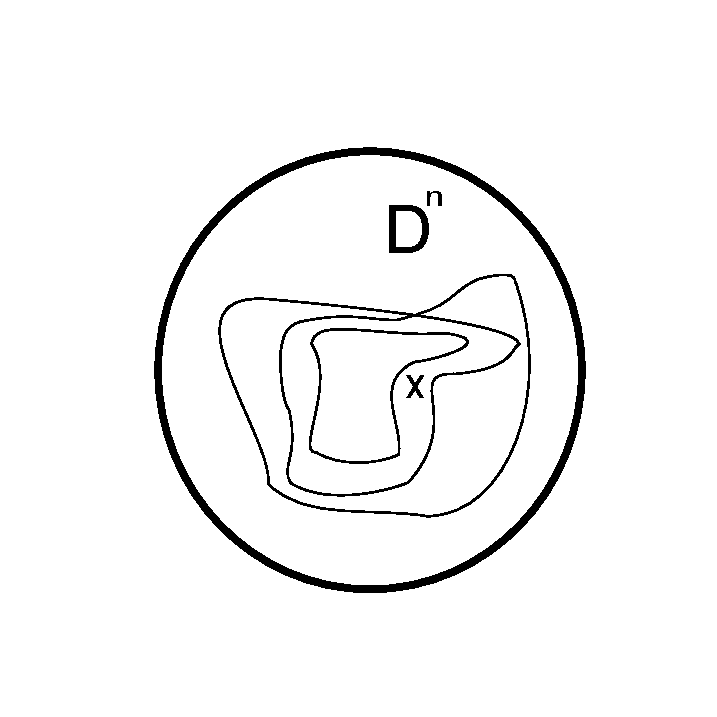
\includegraphics[width=0.2\textwidth]{figures/26.pdf}
%\caption{\small Set-up for Milnor-Spanier duality.}
%\end{wrapfigure}
Take $X \subseteq \mathrm{int}(D^n) \cong \Rbb^n$, and suppose $N \subseteq \mathrm{int}(D^n)$ is a regular neighborhood,\footnote{If you embed a finite complex into a Euclidean space, any sufficiently small
open neighborhood admits a deformation retraction back to the complex
 --- this is a `regular neighborhood'. If the complex is a manifold,
you can identify the normal bundle of the embedding with a regular
neighborhood. } so that the inclusion $X \xrightarrow{\simeq} N$ is a homotopy equivalence.  Then $D(\Xpt) \simeq \Suspend^{1-n}(D^n - N)$, by Alexander duality.
The virtue of the regular neighborhood is that you can identify what the suspension of the complement is: all you need to find the suspension is an inclusion into a contractible space, which we have, giving a degenerate cofiber sequence:
\begin{ctikzcd}
(D^n - N) \rar & D^n \rar &  D^n/(D^n - N) \rar["\simeq"] & \Suspend(D^n - N)\rar & \Sigma D^n
\end{ctikzcd}
Thus, as $D^n/(D^n-N)$ is homeomorphic to $\overline N/\partial\overline N$,
\[D(X_+)\simeq\Suspend^{1-n}(D^n - N) \simeq \Suspend^{-n}(D^n / (D^n-N)) \simeq \Suspend^{-n}(\bar N / \partial \bar N).\]
This is most useful when you can say something about $N$.  If $X$ is a $d$-dimensional manifold without boundary, then the normal bundle $\nu$ of the inclusion $X \into D$ is $(n-d)$-dimensional and $N$ is homotopy equivalent to the disk bundle of $\nu$.  It follows that $\bar N / \partial \bar N$ models the Thom complex $T (\nu)$, so $D(\Xpt) \simeq \Suspend^{-n} T(\nu) \simeq T(\nu - n \varepsilon)$.  This is called ``Milnor-Spanier duality'' (although it's not called that very often).  In (co)homology,
\[
E^{-i}(\Xpt) = E_i (D(\Xpt)) = E_{i+n} (T (\nu)).
\]
Observe also that $\nu + \tau = n \varepsilon$ where $\tau$ is the tangent bundle, so $D(\Xpt) = T(\nu - n \varepsilon) = T(-\tau)$, giving
\[
E^{-i}(\Xpt) = E_i (D(\Xpt)) = E_{i} (T (-\tau)).
\]
\subsection*{Poincar\'e duality}
If $\nu$ (or equivalently, $\tau$) is oriented for $E$ in the Milnor-Spanier setup, then the Thom isomorphism says $E_{i+n} (T (\nu)) \cong E_{i+d} (\Xpt)$. Thus:\footnote{More abstractly: the Thom isomorphism gives $E_{i-d}(T(-\tau))\cong E_i(X_+)$, and $E^{d-i}(X_+)\cong E_{i-d}(T(-\tau))$ by Milton-Spanier.}
\[E^{-i} (\Xpt) \cong E_{i+d} (\Xpt).\]
This gives standard Poincare duality, recalling that $E$ stands for the \emph{reduced} cohomology theory.

\subsection*{Atiyah duality}
%\begin{wrapfigure}[13]{r}{0.3\textwidth}
%\centering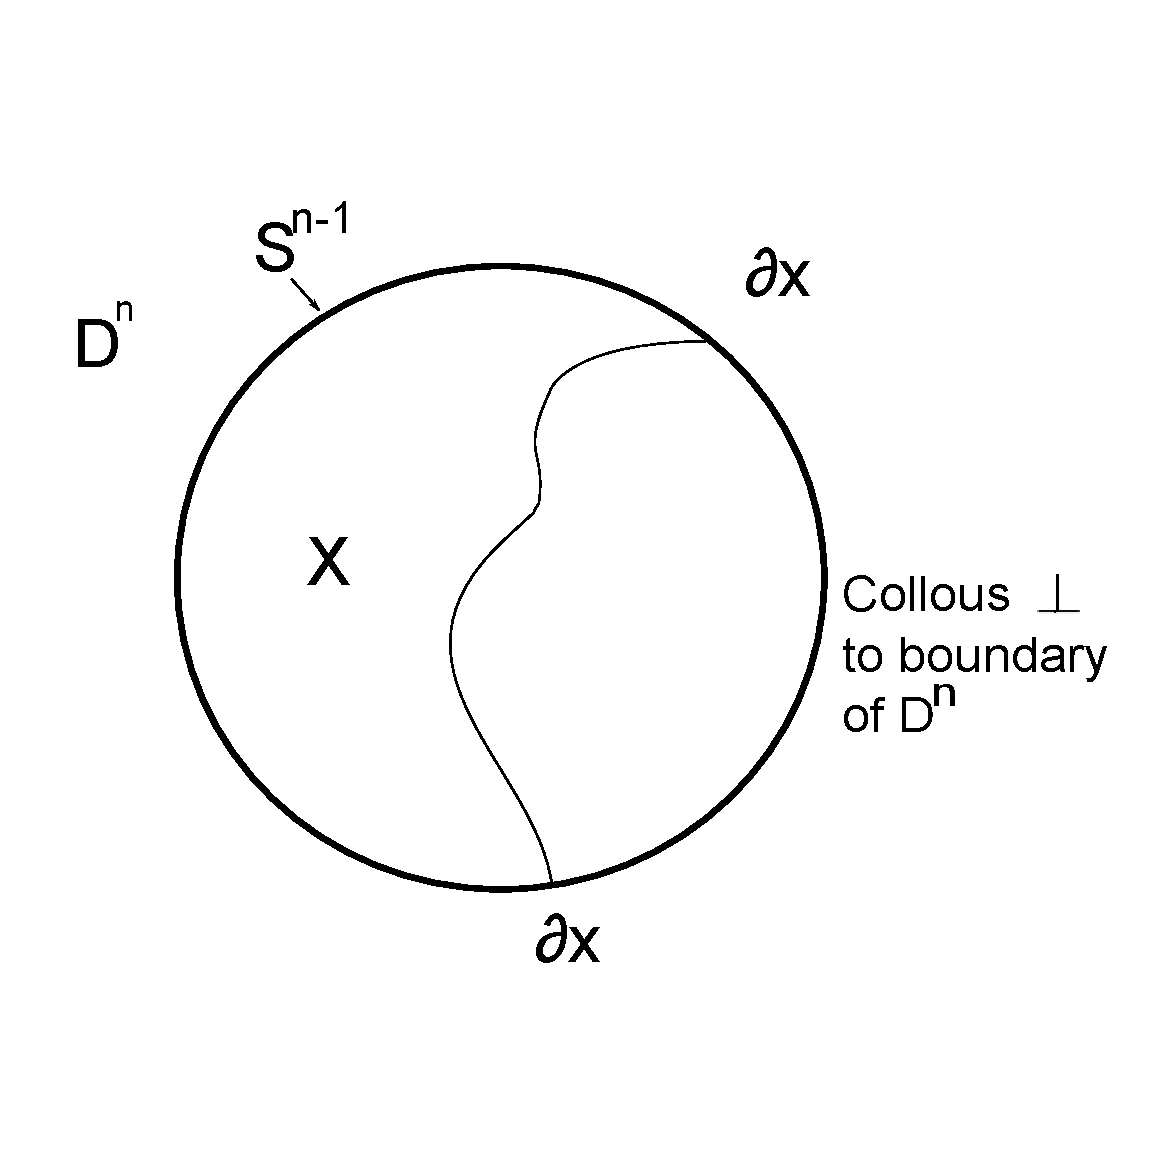
\includegraphics[width=0.3\textwidth]{figures/28.pdf}\vspace{-1cm}
%\caption{\small Diagram of Atiyah duality.}
%\end{wrapfigure}
This is a little mystical, so perhaps we should look at it more closely in the context of what's called Atiyah duality (for this, readers should look at Atiyah's exposition~\cite{Atiyah}).  Here we take for a change $(X, \partial X)$ to be a manifold with boundary.  You have to be careful about interpreting the tangent bundle of a manifold with boundary; $\tau_X$ is best defined to be $d$-dimensional everywhere, but with an identified $(d-1)$-dimensional subbundle on the boundary.  %Referencing the figure, this isn't quite what we had before.

Now suppose that $X$ is embedded in $D^n$ such that $\partial X$ lies in $\partial D^n=S^{n-1}$, and moreover that $X$ is transverse to $S^{n-1}$ wherever they coincide. Suppose also that $N$ is an open neighborhood of $X$ in $D^n$ such that $N\cap S^{n-1}$ is a regular open neighborhood of $\partial X$ in $S^{n-1}$. Then, we take the cone on this situation, as in figure \ref{AtiyahDuality}.
\begin{figure}[ht!]
\centering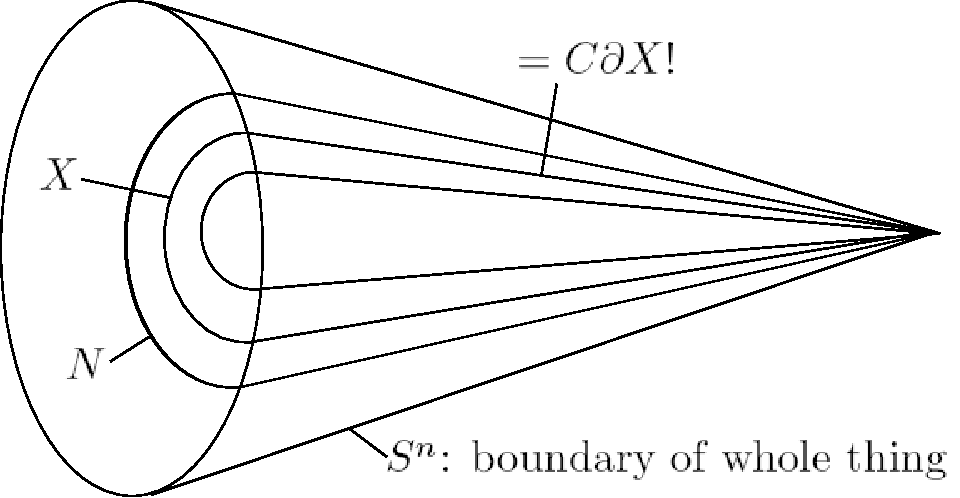
\includegraphics[width=0.4\textwidth]{figures/figure29.pdf}
\caption{\small Atiyah duality.}\label{AtiyahDuality}
\end{figure}

Now, $X / \partial X$ is homotopic to  $Y = X \cup C \partial X$, which is a subcomplex of $\partial(CD^n)\cong S^n$.  Moreover, $Y$ has $N \cup C(N \cap S^{n-1})$ as a regular neighborhood in $S^n$, and its complement is $K=S^n - (N \cup C(N \cap S^{n-1}))$.  Finally, $K$ deformation retracts onto $(D^n-N)$, as the tip of the cone does not lie in $K$. So, applying Alexander duality to $Y\subseteq S^n$ gives
\begin{align*}
D(X / \partial X) & \simeq D(Y) \\
& \simeq \Suspend^{1-n}(K) \\
& \simeq \Suspend^{1-n}(D^n - N) \\
& \simeq \Suspend^{-n}(\bar N / \partial \bar N) \\
& \simeq \Suspend^{-n} T (\nu)\\
& = T(-\tau),
\end{align*}
and this is Atiyah duality.

Now suppose $X$ is a compact closed manifold and $\xi \downarrow X$ is a smooth vector bundle; then $(D(\xi), S(\xi))$ is a compact manifold with boundary.  Atiyah duality says
\begin{align*}
D(T(\xi))
& \simeq T(-\tau_{D(\xi)}) \\
& \simeq T(-\pi^*(\tau_X \oplus \xi)) \\
& = T(-\tau_X - \xi),
\end{align*}
where $\pi$ is the projection $D(\xi) \to X$ (a homotopy equivalence).
\subsection*{Lefschetz duality}
Now suppose that $X$ is oriented for $E$, i.e., that there is a Thom isomorphism $E_i(X_+)\cong E_{i-d}(T(-\tau))$. Then from Atiyah duality we derive Lefschetz duality: $E_i (X_+) \simeq E^{d-i}(X, \partial X)$.
\subsection*{Stunted projective space}
Here's an example: take $X = \RP^{k-1}$ and $\xi = n \bundle{L}$. % (we'll take $n \ge 0$ for the moment; we'll see it doesn't make any difference soon).
Then, we saw in lecture \ref{BuildingThomSpaces} (at least for $n\geq0$) that \[T(n \bundle{L}) = \RP^{n+k-1} / \RP^{n-1} =: \RP^{n+k-1}_n.\]
More generally, we can define, whenever $t+b\geq1$:
\[\RP^{t-1}_{-b}:= T(-bL\downarrow\RP^{t+b-1}),\]
a spectrum with cells in every dimension from $-b$ to $t-1$, inclusive.

Moreover, it happens\footnote{To see this, one argues as follows. View $\bundle{L}$ as a subbundle of $\RP^{k-1}\times \Rbb^k$, where $\RP^{k-1}$ is viewed as the set of lines $\Rbb\{x\}$ in $\Rbb^k$, for nonzero $x\in\Rbb^k$. Then we can produce a bundle isomorphism $\Hom(\bundle{L},\bundle{L}^\perp)\to\tau(\RP^{k-1})$ by sending $h:\Rbb\{x\}\to \Rbb\{x\}^\perp$ to the germ at $0$ of the path $t\mapsto \Rbb\{x+t\cdot h(x)\}$ in $\RP^{k-1}$. Noting that $\Hom(\bundle L,\bundle L)$ is a line bundle with a nonvanishing section, it is trivial, so $\tau(\RP^{k-1})+\Rbb=\Hom(\bundle L,\bundle L^\perp\oplus\bundle L)=\Hom(\bundle L,\Rbb^k)=\Hom(\bundle L,\Rbb)^k=\bundle L^k$.}\todo{I find this footnote very hard to read.} that $\tau(\RP^{k-1}) + \varepsilon = k \bundle{L}$.
%\begin{enumerate}
%\item $T(n \bundle{L}) = \RP^{n+k-1} / \RP^{n-1} \simeq \RP^{n+k-1}_n$, (see lecture); and
%\item $\tau(\RP^{k-1}) + \varepsilon = k \bundle{L}$.\footnote{To see this, one argues as follows. View $\bundle{L}$ as a subbundle of $\RP^{k-1}\times R^k$, where $\RP^{k-1}$ is viewed as the set of lines $\Rbb\{x\}$ in $\Rbb^k$, for nonzero $x\in\Rbb^k$. Then we can produce a bundle isomorphism $\Hom(\bundle{L},\bundle{L}^\perp)\to\tau(\RP^{k-1})$ by sending $h:\Rbb\{x\}\to \Rbb\{x\}^\perp$ to the germ at $0$ of the path $t\mapsto \Rbb\{x+t\cdot h(x)\}$ in $\RP^{k-1}$. Noting that $\Hom(\bundle L,\bundle L)$ is a line bundle with a nonvanishing section, it is trivial, so $\tau(\RP^{k-1})+\Rbb=\Hom(\bundle L,\bundle L^\perp\oplus\bundle L)=\Hom(\bundle L,\Rbb^k)=\Hom(\bundle L,\Rbb)^k=\bundle L^k$.}
%\end{enumerate}
By Atiyah duality, $D(T(n\bundle{L})) \simeq T(-n \bundle{L} - \tau)$, so that
\[D(\RP^{n+k-1}_n) = D(T(n\bundle{L})) \simeq T(-n \bundle{L} - \tau) = T(-n \bundle{L} + \varepsilon -k \bundle{L}) = \Suspend T(-(n+k)\bundle{L}) =: \Suspend \RP^{-n-1}_{-n-k}.\]
Summarizing:
\[D(\RP^{t-1}_{-b}) \simeq \Suspend (\RP^{b-1}_{-t})\text{ for }t+b\geq1.\]
% $D(\RP^{t-1}_{-b}) \simeq \Suspend \RP^{b-1}_{-t}$, for $b, t \in \Zbb$, $t-1 \ge -b$ (and taking $b = -n$, $t = n+k$ in the above.  The condition $t-1 \ge -b$ requires that $\RP^{t-1}_{-b}$ has a cell.) or $\RP^{t-1}_b = T(-b \bundle{L} \downarrow \RP^{t+b-1})$.

By the way, if you don't like these somewhat ethereal spaces, you can use James Periodicity: let $a$ be the periodicity of $\bundle{L}$ in $\widetilde J(\RP^{t+b-1})$.  Then $T((ja-b)\bundle{L}) \simeq \Suspend^{ja} T(-b \bundle{L})$; for $j$ big enough, $T((ja-b)\bundle{L})$ is an actual stunted projective space!

% >>>
\fi
\BoxedNote{}












\section{The structure of stunted projective space} % <<<
\label{TheStructureOfStuntedProjectiveSpace}
\ifx\OutputTheStructureOfStuntedProjectiveSpace\undefined\else
Today we look at the attaching maps for stunted projective spaces.  In fact, the attaching maps we're going to look at are the ``stable relative attaching maps,'' so perhaps we should begin by saying what that means.  Suppose $X$ is a CW complex; then it has a skeletal filtration $\Sk_* (X)$.  The $(k+1)$-skeleton is obtained from the $k$-skeleton by attaching $(k+1)$-cells as in the following pushout square:
\begin{ctikzcd}
\Sk_k (X) \rar[hook] & \Sk_{k+1} (X) \\
\bigvee S^k \uar\rar[hook] & \bigvee D^{k+1}\uar.
\end{ctikzcd}
Although the attaching maps $S^k \to \Sk_k (X)$ are to the $k$-skeleton, it's certainly possible that an attaching map pulls back to a lower skeleton.  A ``relative attaching map'' for a $(k+1)$-cell (attached via $r$) is a factorization of this kind through the lowest possible skeleton; that is, the map $a'$ below:
\begin{ctikzcd}[column sep=large]
\Sk_{k-j-1} (X) \rar[into] & \Sk_{k-j} (X)  \rar[hook,"\cdot\,\cdot\,\cdot" description] & \Sk_k (X) \rar[into] & \Sk_{k+1} (X)\\
&S^k\ular[dashed,"\nexists" scale=1.5]\uar["a'"]\urar[yshift=0.2em,"r"]\rar[into]&\bigvee S^k\uar\rar[into]&\bigvee D^{k+1}\ar[u]
\end{ctikzcd}
A ``stable relative attaching map'' is a stable one of these.  That is, the cells of the $(k+2)$-skeleton of $\Suspend X$ are the suspension of the cells of the $(k+1)$-skeleton of $X$,
so one could ask how far down an attaching map factors, perhaps after suspending very often (ignoring the wavy arrow for the moment):
\begin{ctikzcd}[column sep=large, decoration={markings, mark connection node=dots, mark=at position .5 with {\node (dots) {$\cdots$};}}]
&\bigvee S^{k-j+n}\mathrlap{=C(\imath)}\\
\Sk_{k-j+n-1} (X) \rar[into] & \Sk_{k-j+n} (X) \uar[wavy,"b"'] \rar[hook,"\cdot\,\cdot\,\cdot" description] & \Sk_{k+n} (X) \rar[into] & \Sk_{k+n+1} (X)\\
&S^{k+n}\ular[dashed,"\nexists" scale=1.5]\ar[u,"a'"]\urar[yshift=0.1em,"r"]\rar[into]&\bigvee S^{k+n}\uar\rar[into]&\bigvee D^{k+n+1}\ar[u]
\end{ctikzcd}
The inclusion $\imath$ of one skeleton in the next is a cofibration, and stably, the corresponding cofibration sequence (drawn with the wavy arrow $b$) is also a fibration sequence.
Thus, if $a$ does not factor stably through a lower skeleton the composite $ba$ defines a nonzero element of $\pi_{k+n}^S \left( \bigvee S^{k-j+n} \right) = \bigoplus \pi_j^S$.\footnote{Warning: there's indeterminacy in how you factor the attaching map, so the element you get may not be well-defined.}

In any case, we want to understanding the stable relative attaching maps for $\RP^\infty$ using the standard cell structure, with one cell in each dimension. We'll format the diagrams a little differently now. Let $\pi$ be the attaching map for a particular cell in dimension $k$  and let $c$ be the collapse map from $\RP^{k-j}$ onto its top cell.

In the following diagram we ask for the largest value of $j$ such that the stable attaching map factors, and also what the compression $c\overline\pi$ of the stable attaching map onto the top cell is as an element of $\pi^S_j$.
\begin{ctikzcd}[column sep = 4.5em,row sep=2.3em]
\RP^{k-j-1}\ar[from=drrr,dashed,"\nexists" {very near end, scale=1.5}]\rar[hook,"\imath"] & \RP^{k-j}\dar[crossing over, "c"' pos=0.6]\rar[hook,"\cdot\,\cdot\,\cdot" description] & \RP^k \rar[hook] & \RP^{k+1}\\
&S^{k-j}&&\ar[ull,"\overline\pi"' pos=0.53]S^{k}\ar[ul,"\pi"']\ar[ll,"c\overline\pi"]
\end{ctikzcd}

%\begin{ctikzcd}[row sep=large, column sep = 4em]
%\RP^{k-j-1}\ar[from=drr,dashed,"\nexists" {near end, scale=1.5}]\rar[hook,"\imath"] & \RP^{k-j}\dar[crossing over,"c" pos=0.4]\rar[hook,] & \RP^k \rar[hook] & \RP^{k+1}\\
%&S^{k-j}&\ar[ul,"\overline\pi"']S^{k}\ar[u,"\pi"']\ar[l,"c\overline\pi"]
%\end{ctikzcd}

The answer will come out in terms of the image of the $J$-homomorphism --- actually its stable version $j: \pi_{*-1}(O) \to \pi_{*-1}(QS^0) = \pi_{*-1}^S$.  Remember $\pi_{*-1}(O) = \pi_* (BO) = \KOtwee^{-*}$.  Here's a table, leaving out degrees where $\KOtwee^{-*} = 0$:

\[
\begin{array}{cc|ccl}
i=\nu(2^i) & *=\rho(2^i) & \KOtwee^{-*}=\pi_{*-1}(O) &&j_i:=j(g_i)\in\pi_{*-1}^S \\
\hline
0 & 1 & {\Zbb_2 \anglebrace{g_0}} && j_0=-2 \iota \\
1 & 2 & {\Zbb_2 \anglebrace{g_1}} && j_1=\eta \\
2 & 4 & {\phantom{_2}\Zbb \anglebrace{g_2}} && j_2=\nu\ %\{
\smash{\Biggr \}
\raisebox{-1.1ex}{\small\shortstack{Hopf invariant\\one elements}}}\\
3 & 8 & {\phantom{_2}\Zbb \anglebrace{g_3}} && j_3=\sigma \\
4 & 9 & {\Zbb_2 \anglebrace{g_4}} && j_4=\eta \sigma \\
5 & 10 & {\Zbb_2 \anglebrace{g_5}} && j_5=\eta^2 \sigma
\end{array}
\]

Implicit in the organization of this table is the observation that the coefficient groups $\KOtwee^{-*}$ are all cyclic, and nonzero only when $*=\rho(2^e)$. Thus we write $g_i$ for a generator of the $(i+1)^\text{st}$ nonzero coefficient group, and $j_i$ for its image $j(g_i)$ under the stable $J$-homomorphism.

Note that $g_0$ has order two, but $j_0:=j(g_0)$ has infinite order, so that $j:\pi_0(O)\to\pi^S_0$ cannot be a homomorphism. However, it is a homomorphism in higher degrees.\todo{This remark will go away when we replace $QS^0$ with $BGL_1 \Sbb^0$.}

Our discussion of the attaching maps will begin where the answer is, which may seem like a funny place at first, so have patience.  Recall the following facts:
\[\KOtwee(\RP^k)=\Zbb_{a_k}\anglebrace{\bundle L-1},\text{ defining }\begin{array}{c|cccccccc}
k&0&1&2&3&4&5&6&7\\\hline
a_k&1&2&4&4&8&8&8&8
\end{array}\text{ and }a_{k+8}=16a_k,\]
so that, $a_k|n$ exactly when $k\leq\rho(n)-1$. Thus when $k = \rho(n) - 1$ we have $a_k=2^{\nu(n)}$ and $a_{k+1}=2^{\nu(n)+1}$. Just to reiterate the above, this gives
\begin{align*}
\KOtwee \left( \RP^{\rho(n) - 1} \right) & = \Zbb_{2^{\nu(n)}} \anglebrace{\bundle L - 1 } \\
\KOtwee \left( \RP^{\rho(n)} \right) & = \Zbb_{2^{\nu(n) + 1}} \anglebrace{\bundle L - 1 }.
\end{align*}
Now note that $\imath^*(\bundle L)=\bundle L$, where $i$ is the inclusion in the cofiber sequence
\begin{tikzcd}[column sep=scriptsize]
\RP^{\rho(n) - 1} \rar[into,"\imath"]& \RP^{\rho(n)} \ar[r,"b"]& S^{\rho(n)}
\end{tikzcd}.
We then examine the exact sequence
\begin{ctikzcd}
\KOtwee \left( \RP^{\rho(n) - 1} \right) & \lar["\imath^*"'] \KOtwee \left( \RP^{\rho(n)} \right) & \lar["b^*"'] \KOtwee (S^{\rho(n)})\\
\Zbb_{2^{\nu(n)}} \anglebrace{\bundle L - 1 }\uar[equal] & \lar[onto,"\imath^*"']\Zbb_{2^{\nu(n) + 1}} \anglebrace{\bundle L - 1 }\uar[equal] & \lar["b^*"']\anglebrace{g_{\nu(n)}}\uar[equal].
\end{ctikzcd}
By exactness, $b^*(g_{\nu(n)})=2^{\nu(n)}(\bundle L - 1)=n(1-\bundle L)$, the nonzero element\footnote{Notice that in $\Zbb_{2^{\nu(n) + 1}} \anglebrace{\bundle L - 1}$, $2^{\nu(n)}(\bundle L - 1)$ is congruent to any of its odd multiplies, and $-n$ is an odd multiple of $2^{\nu(n)}$.} of $\ker(\imath^*)\simeq\Zbb_2$.
%That is $b^*(g_{\nu(n)})=n(\bundle L-1)$.

In terms of bundles, this means that $n(1-\bundle L)$ over $\RP^{\rho(n)}$ is classified by a map into $BO$ that factors as $b$ followed by $g_{\nu(n)}$:
\begin{center}
\begin{tikzcd}
\ar[d]n(1-\bundle L) \ar[r] & E(g_{\nu(n)})\ar[d] \\
\RP^{\rho(n)}\rar["b"] & S^{\rho(n)} \rar["g_{\nu(n)}"] & BO
\end{tikzcd}
%
\quad
%
\sbox0{\Bullet $E(g_{\nu(n)})$ is the virtual bundle classified by $g_{\nu(n)}$}
\begin{minipage}{\wd0}
\Bullet $E(g_{\nu(n)})$ is the virtual bundle classified by $g_{\nu(n)}$

\Bullet $H^{\rho(n)}(b;\Zbb_2)$ is an isomorphism
\end{minipage}
%
%\fbox{\begin{minipage}{5cm}
%\Bullet $E(g_{\nu(n)})$ is the virtual bundle classified by $g_{\nu(n)}$
%
%\Bullet $H^{\rho(n)}(b;\Zbb_2)$ is an isomorphism
%\end{minipage}}
\end{center}
That's the starting point.  Now we study the Thom spaces to get stunted projective spaces.  In the $\Scat$-category, we have a map on Thom spaces (relative to $S^0$):
\begin{ctikzcd}
S^0 \dar\rar[equal] & S^0\dar\\
\Suspend^n\!\left(\RP^{\rho(n)-n}_{-n}\right)\rar["\btwee"] & T\!\left(g_{\nu(n)}\right)
\end{ctikzcd}

The first question is: ``what is $T(g_{\nu(n)})$?''  By the Thom isomorphism, $T(g_{\nu(n)})$ has a 0-cell and a $\rho(n)$-cell; the attaching map is an element of $\pi_{\rho(n)-1} (Q S^0)$.
\begin{thm}
The attaching map for $T(g_{\nu(n)})$ is $j_{\nu(n)} = j(g_{\nu(n)}) \in \pi_{\rho(n)-1}(QS^0)$.
\end{thm}
This almost has the status of a folk theorem; it's due to Toda and Adams.  We will prove it next time; for now, what else could it be?  Now we can line up two cofiber sequences vertically:
\begin{ctikzcd}
S^0 \dar\rar[equal] & S^0\dar\\
\Suspend^n\!\left(\RP^{\rho(n)-n}_{-n}\right)\dar\rar["\btwee"] & T\!\left(g_{\nu(n)}\right)\dar\\
\Suspend^n\!\left(\RP^{\rho(n)-n}_{-n+1}\right)\rar["c"] & S^{\rho(n)}
\end{ctikzcd}
Now $\Suspend^n (\RP^{\rho(n)-n}_{-n+1})$ has a cell in each dimension from 1 to $\rho(n)$ inclusive. By naturality of the Thom isomorphism $H^{\rho(n)}(\widetilde b;\Zbb_2)$ is an isomorphism in dimension $\rho(n)$,  so the 5-lemma implies that $H^{\rho(n)}(c;\Zbb_2)$ is also an isomorphism, and $c$ is the collapse map (up to sign).
\ConfusedBox{Must we localize at two to assert this about $c$?}
In other words, $\Suspend^n \RP^{\rho(n)-n}_{-n}$ has cells between dimensions $0$ and $\rho(n)$, and the map to $T(g_{\nu(n)})$ strips away the cells in between.
\begin{figure}[h!]
\centering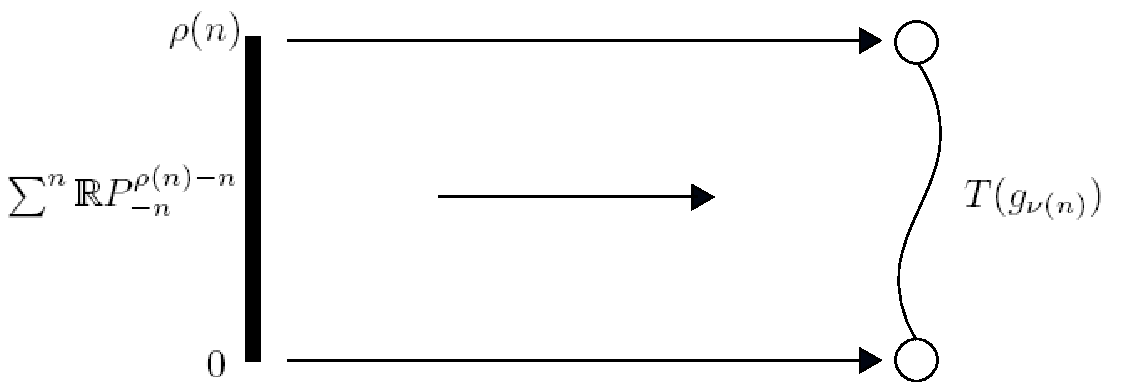
\includegraphics[width=0.4\textwidth]{figures/figure30.pdf}
\caption{\small Picture of the map $\widetilde b$.}
\end{figure}

Well that's pretty good, only attaching maps are supposed to go the other way, so let's dualize this picture.  Two facts about the Spanier-Whitehead dual we will use are that $D \RP^{t-1}_{-b} = \Suspend \RP^{b-1}_{-t}$ (see lecture \ref{Dualities}), and that the dual $D(f)$ of $f:S^p\to S^0$ is $\pm\Sigma^{-p}f:S^0\to S^{-p}$.

The only space whose dual we have left to compute is $T(g_{\nu(n)})$.  Since by the folk theorem $T(g_{\nu(n)}) = C(j_{\nu(n)})$ we have a cofiber sequence
\begin{tikzcd}[column sep=normal]
S^{\rho(n)-1} \rar["j_{\nu(n)}"] & S^0 \rar& T(g_{\nu(n)}).
\end{tikzcd}
Continuing the dual cofiber sequence:
\begin{ctikzcd}
\Sigma^{-\rho(n)+1}T(g_{\nu(n)}) & \lar S^{-\rho(n)+1}
&[-\columnsep+1em+width("${}^{\pm\Sigma^{-\rho(n)+1}j_{\nu(n)}}$")]
\lar["\pm\Sigma^{-\rho(n)+1}j_{\nu(n)}"'] S^0 & \lar D(T(g_{\nu(n)}))
\end{ctikzcd}
Thus $D(T(g_{\nu(n)}))=\Suspend^{-\rho(n)}T(g_{\nu(n)})$, so $T(g_{\nu(n)})$ is nearly self-dual. In particular, we can now write down the dual diagram to that drawn above\todo{Make it more explicit which diagram above.} (at left) and its $(n-1)$-fold suspension (at right):
\begin{cjointikzcd}[sep=large]
\diagram
    S^0 \rar[equal] & S^0\\
    \Sigma^{1-n}\RP^{n-1}_{n-\rho(n)-1}\uar& \lar["D\btwee"'] \Sigma^{-\rho(n)}C\left(j_{\nu(n)}\right)\uar\\
    \Sigma^{1-n}\RP^{n-2}_{n-\rho(n)-1}\uar & \lar["Dc"' pos=0.67] S^{-\rho(n)}\uar\\
    S^{-1}\uar \rar[equal] & S^{-1}\uar["\Sigma^{-\rho(n)}j_{\nu(n)}"]
%
\diagram
    S^{n-1} \rar[equal] &[width("$C\left(j_{\nu(n)}\right)$")] S^{n-1}\\
    \RP^{n-1}_{n-\rho(n)-1}\uar&\lar["\Sigma^{n-1}D\btwee"'] \Sigma^{n-\rho(n)-1}\edgerlap{C\left(j_{\nu(n)}\right)}\uar\\
    \RP^{n-2}_{n-\rho(n)-1}\uar & \lar["\Sigma^{n-1}Dc"'] S^{n-\rho(n)-1}\uar\\
    S^{n-2}\uar \rar[equal] & S^{n-2}\uar["\Sigma^{n-\rho(n)-1}j_{\nu(n)}"]
\end{cjointikzcd}
\todo[noline]{I think we should suppress the suspensions from the arrow names in the righthand diagram.}
Here, $\pi$ is the attaching map for $\RP^{n-2}_{n-\rho(n)-1} \to \RP^{n-1}_{n-\rho(n)-1}$; this follows because the columns are cofiber sequences. Moreover, as $\Sigma^{n-1} Dc$ is dual to the collapse map (up to sign), it is the inclusion of the bottom cell (up to sign). %  The map $j_{\nu(n)}$ might look funny, but it works out because we're dealing with spectra.
Well so we've done it: we've factored $\pi$ as $j_{\nu(n)}$ followed by inclusion of the bottom cell.
\begin{ctikzcd}
S^{n-2}\drar["j_{\nu(n)}"] \rar["\pi"] & \RP^{n-2}_{n-\rho(n)-1} \\
& S^{n-\rho(n)-1}\uar
\end{ctikzcd}
In other words, the attaching map for the top cell of $\RP^{n-1}_{n-\rho(n)-1}$ pulls all the way back to the $(n-\rho(n)-1)$-skeleton.  It goes no further: that would mean that $\pi \simeq \ptspace$, but if $\pi$ were stably nullhomotopic, then the top cell of $\RP^{n-1}_{n-\rho(n)-1}$ would stably split off. Dualizing, the bottom cell $S^0$ of $\Suspend^n \RP^{\rho(n)-n}_{-n} = T(n(1-\bundle L) \downarrow \RP^{\rho(n)})$ would split off, which would then imply that $n(1-\bundle L)$ would be stably fiber homotopy trivial. This is of course not the case, by the solution to the vector fields problem --- $\widetilde J (\RP^{\rho(n)}) = \Zbb_{2^{\nu(n)+1}} \anglebrace{\bundle L - 1 }$.

\ConfusedBox{\textbf{For some reason I find this a bit confusing. I've put in an alternative.} It goes no further: that would mean that $\pi \simeq \ptspace$, but if $\pi$ is stably nullhomotopic then we'd get
\begin{ctikzcd}[ampersand replacement=\&]
\& \& S^0\dlar["\exists"]\dar["\id"] \\
\Suspend^{-n+1} \RP^{n-2}_{n - \rho(n) - 1} \rar \& \Suspend^{-n+1} \RP^{n-1}_{n-\rho(n)-1} \rar \& S^0 \rar["\pi"] \& \Suspend^{-n+2} \RP^{n-2}_{n-\rho(n)-1},
\end{ctikzcd}
because the sequence is an exact triangle, a map going back as above.  Looking at what that means in terms of the dual, it means there is a stable splitting of the $0$-sphere \begin{tikzcd}[ampersand replacement=\&,column sep=scriptsize]
S^0 \rar[yshift=0.2em] \& \lar[yshift=-0.2em] \Suspend^n \RP^{\rho(n)-n}_{-n} = T(n(1-\bundle L) \downarrow \RP^{\rho(n)})
\end{tikzcd} which would mean that $n(1-\bundle L)$ is stably fiber-homotopy trivial, equivalently that $n\bundle L$ is stably fiber-homotopy trivial.  But by the vector field problem, it's not: $n(1-\bundle L) \ne 0$ in $\widetilde J \RP^{\rho(n)} = \Zbb_{2^{\nu(n)+1}} \anglebrace{\bundle L - 1 }$.
}
Now it's an easy matter to get back to the general case: consider $\RP^{n-1}_{-N}$, where $-N \leq n - \rho(n) - 1$.\footnote{The quantity $n - \rho(n) - 1$ is $-1$ when $n=1,2,4,8$, and positive for other $n>0$.}   Then we have a diagram with the bottom row a cofiber sequence (drawn at left):
\begin{cjointikzcd}[intertext,row sep=tiny]
\diagram
& \RP^{n-2}_{-N}\rar["\text{coll}" pos=0.65] & \RP^{n-2}_{n-\rho(n)-1}\\
\RP^{n-\rho(n)-2}_{-N} \rar[into]   & \RP^{n-\rho(n)-1}_{-N} \rar["\text{coll}" pos=0.45] \uar[hook] & S^{n-\rho(n)-1}\uar[hook]
%
\diagram[1em] \intertext{Applying $\pi_{n-2}^S(\text{---})$:}
%
\diagram[-8em] % There seems to be a bug in cjointikzcd.
& \pi\rar[mapsto] & \pi\\
? \rar[mapsto,dashed] & \overline\pi \rar[mapsto]\uar[mapsto] & j_{\nu(n)}\uar[mapsto]
\end{cjointikzcd}
From what we had before, the attaching map $\pi:S^{n-2}\to\RP^{n-2}_{-N}$ pulls back stably to a map $\overline\pi:S^{n-2}\to\RP^{n-\rho(n)-1}_{-N}$, whose compression onto the top cell $S^{n-\rho(n)-1}$ is $j_{\nu(n)}\neq0$. Thus, applying $\pi_{n-2}^S$ to the above diagram, we have elements as in the box at the right. As $j_{\nu(n)}$ is nonzero, and the bottom row is exact ($\pi_*^S$ is a homology theory) there can be no element of $\pi_{n-2}^S(\RP^{n-\rho(n)-2}_{-N})$ mapping to $\overline \pi$.
Thus:
\begin{thm}\label{RelAttachThm}
The stable relative attaching map for the $(n-1)$-cell of $\RP^{n-1}_{-N}$ can be taken to be $j_{\nu(n)}$; that is, stably, there is some $\overline \pi$ which does not pull back any further stably, and so that $c\overline\pi=j_{\nu(n)}$:
\begin{ctikzcd}[column sep = 4.5em,row sep=2.3em]
\RP^{n-\rho(n)-2}_{-N}\ar[from=drrr,dashed,"\nexists" {very near end, scale=1.5}]\rar[hook,"\imath"] & \RP^{n-\rho(n)-1}_{-N}\dar[crossing over, "c"' pos=0.6]\rar[hook,"\cdot\,\cdot\,\cdot" description] & \RP^{n-2}_{-N}  \rar[hook] & \RP^{n-1}_{-N} \\
&S^{n-\rho(n)-1}&&\ar[ull,"\overline\pi"' pos=0.53]S^{n-2}\ar[ul,"\pi"']\ar[ll,"j_{\nu(n)}"]
\end{ctikzcd}\todo[noline]{Fix the notation so that this diagram has roughly the same names as the very similar ones back a few pages. The previous set of diagrams use $k=n+2$ in place of $n$.}
%\[\xymatrix@!0@C=3.5cm@R=1.4cm{
%\RP^{n-\rho(n)-2}_{-N}\ar@{^{(}->}[r]^\imath &\ar[d] \RP^{n-\rho(n)-1}_{-N}\ar|{\ \cdot\ \cdot\ \cdot\ }@{^{(}->}[r]& \RP^{n-2}_{-N} \ar@{^{(}->}[r] & \RP^{n-1}_{-N}\\
%&\makebox[0cm][r]{$C(\imath)=$\,}S^{n-\rho(n)-1}&\ar@{^{(}->}[r]\ar[ul]_{\overline\pi}\ar@{-->}[ull]^(.75){\text{\large$\nexists$}}S^{n-2}\ar@{^{(}->}[r]\ar[u]^\pi\ar[l]^{j_{\nu(n)}}&D^{n-1}\ar[u]
%}\]
\end{thm}

It's time to draw some pictures. First, here are the stable relative attaching maps in $\RP^\infty_{-1}$:
\begin{center}
\begin{tikzpicture}[
    scale=0.5, font=\small,
    every path/.append style={out=90,in=90},
    every node/.append style={execute at begin node=$,execute at end node=$},
    every edge quotes/.style={auto=right}
]
    \foreach \x in {-1,...,9,11,13,...,31}
        \node[below] at (\x,-.6) {\x};
    \foreach \x in {-1,...,31}
        \node at (\x,0) {\Bullet};
    \foreach \x in {0,2,...,30}
		\draw (\x,0) to["2\iota"'] (\x-1,0);
    \foreach \x in {1,9,...,25}
		\draw (\x,0) to["\eta" {pos=0.465, yshift=-0.7ex}]   (\x-2,0);
    \foreach \x in {5,13,...,29}
		\draw (\x,0) to["\eta" yshift=-0.3ex]  (\x-2,0);
    \foreach \x in {3,11,...,27}
		\draw (\x,0) to["\nu"] (\x-4,0);
    \foreach \x in {7,23}
		\draw (\x,0) to["\sigma"]  (\x-8,0);
    \foreach \x in {15}
		\draw (\x,0) to["\eta\sigma"]  (\x-9,0);
    \foreach \x in {31}
		\draw (\x,0) to["\eta^2\sigma"]  (\x-10,0);
\end{tikzpicture}
\end{center}
%\begin{center}
%\begin{tikzpicture}[scale=.95]
%    \foreach \x in {-1,...,9,11,13,...,31}
%        \path (.5*\x,-.3) node[below] {\x};
%    \foreach \x in {-1,...,31}
%        \path (.5*\x,0) node {$\Bullet$};
%    \foreach \x in {0,2,...,30}
%		\draw[->] (.5*\x,0) to[out=90,in=90] node[below] {\small$2\iota$}  (.5*\x-.5,0);
%    \foreach \x in {1,5,...,29}
%		\draw[->] (.5*\x,0) to[out=90,in=90] node[right] {\small$\,\ \eta$}  (.5*\x-1,0);
%    \foreach \x in {3,11,...,27}
%		\draw[->] (.5*\x,0) to[out=90,in=90] node[above] {\small$\nu$}  (.5*\x-2,0);
%    \foreach \x in {7,23}
%		\draw[->] (.5*\x,0) to[out=90,in=90] node[below] {\small$\sigma$}  (.5*\x-4,0);
%    \foreach \x in {15}
%		\draw[->] (.5*\x,0) to[out=90,in=90] node[below] {\small$\eta\sigma$}  (.5*\x-4.5,0);
%    \foreach \x in {31}
%		\draw[->] (.5*\x,0) to[out=90,in=90] node[below] {\small$\eta^2\sigma$}  (.5*\x-5,0);
%\end{tikzpicture}
%\end{center}


%\begin{figure}[h!]
%\centering\includegraphics[width=0.8\textwidth]{figures/fig31fix.png}
%\caption{\small Stable relative attaching maps in $\RP^\infty_{-1}$.}
%\end{figure}

For example, if $n$ is odd then $\rho(n) = 1$, $\nu(n) = 0$.  So the attaching map for the top cell of $\RP^{2k}_{-N}$ is $j_0 = 2\iota$.  For $n-1 = 1$, $3$, or $7$, the relative attaching map is to the $(-1)$-cell --- so if it weren't there, stably these cells wouldn't be attached; these splittings correspond to the Hopf-invariant $1$ elements.

The next picture is a spectral sequence: the Atiyah-Hirzebruch spectral sequence for stable homotopy of $\RP^\infty_{-1}$.  The exact couple comes from:
\begin{ctikzcd}
\cdots \rar[into] & \RP^{k-1}_{-1} \rar[into]\dar["c"] & \RP^{k}_{-1} \rar[into]\dar["c"] & \RP^{k+1}_{-1} \rar[into]\dar["c"] & \cdots\\
& S^{k-1} \ular[wavy,"\pi"] & S^k \ular[wavy,"\pi"] & S^{k+1} \ular[wavy,"\pi"]
\end{ctikzcd}
Here the vertical arrows $c$ are the collapse maps,
% onto the top cells of the $\RP^k_{-1}$,
and the wavy arrows $\pi$ are the attaching maps, so drawn to indicate that they shift degree --- they are in fact map maps $\Sigma^{-1}S^k\to\RP^{k-1}_{-1}$. We can apply $\pi_*^S$ to obtain an exact couple (in which the wavy maps shift degree down by one):
\begin{ctikzcd}
\cdots \rar[into] & \pi_*^S(\RP^{k-1}_{-1}) \rar[into]\dar["c"] & \pi_*^S(\RP^{k}_{-1}) \rar[into]\dar["c"] & \pi_*^S(\RP^{k+1}_{-1}) \rar[into]\dar["c"] & \cdots\\
& \pi_*^S(S^{k-1}) \ular[wavy,"\pi"] & \pi_*^S(S^k) \ular[wavy,"\pi"] & \pi_*^S(S^{k+1}) \ular[wavy,"\pi"]
\end{ctikzcd}
From this exact couple we obtain a spectral sequence as usual. It isn't totally clear to what this spectral sequence converges.  However, the restriction principle applies, so any finite piece will converge to $\pi_*^S (\RP^N_{-1})$. The columns at $E_1$ are $\pi_*^S$. That is:
\[E^1_{pq}=\pi^S_{p+q}(S^p)=\pi^S_q.\]
As in the EHP sequence, the differentials record how far back you can pull a class.  So our stable relative attaching maps tell us about non-zero differentials in this spectral sequence.

The differential $d_r$ is defined as usual, that is, if $[x]\in E_{pq}^r$ is a class with representative $x\in\pi^S_{p+q}(S^p)$, then $\pi(x)\in\pi^S_{p+q-1}(\RP^{p-1}_{-1})$ pulls back to an element $y\in \pi^S_{p+q-1}(\RP^{p-r}_{-1})$, and $cy\in \pi^S_{p+q-1}(S^{p-r})$ represents an element of $E_{p-r,q+r-1}^r$, which is our definition of $d_r([x])$.

Consider the element $\iota\in E^1_{p-1,0}=\pi^S_{p-1}(S^{p-1})$, and its fate in the spectral sequence. Now $\pi(\iota)\in \pi^S_{p-2}(\RP^{p-2}_{-1})$ is simply the attaching map for the $(p-1)$-cell. Thus, theorem \ref{RelAttachThm} can be rephrased:
\begin{thm}
The differentials $d_r$ vanish on $[\iota]\in E_{n-1,0}^r$, for $r\leq\rho(n)-1$, and $d_{\rho(n)}[\iota]=[j_{\nu(n)}]$, a nonzero element of $E^{\rho(n)}_{n-\rho(n)-1,\rho(n)-1}$.
\end{thm}
We illustrate this theorem with the following picture of the nonzero differentials which occur on the fundamental classes on the bottom row of the spectral sequence:
\begin{center}
\begin{tikzpicture}[
    scale=0.5, font=\small,
    every path/.append style={->},
    every node/.append style={execute at begin node=$,execute at end node=$},
    every edge quotes/.style={auto=right,inner sep=1pt}
]
    \foreach \x in {-1,...,9,11,13,...,31}
        \node[below,font=] at (\x,-.4)  {\x};
    \foreach \y in {0,...,9}
        \node[left,font=] at (-1.4,\y) {\y};
    \foreach \x in {-1,...,31}
    \foreach \y in {0,...,9}
		\node[font=\tiny] at (\x,\y)  {\cdot};
    \foreach \x in {0,2,...,30}
		\draw (\x,0) to["2\iota" inner sep=2pt]  (\x-1,0);
    \foreach \x in {1,5,...,29}
		\draw (\x,0) to["\eta"]  (\x-2,1);
    \foreach \x in {3,11,...,27}
		\draw (\x,0) to["\nu"]  (\x-4,3);
    \foreach \x in {7,23}
		\draw (\x,0) to["\sigma"]  (\x-8,7);
    \foreach \x in {15}
		\draw (\x,0) to["\eta\sigma"]  (\x-9,8);
    \foreach \x in {31}
		\draw (\x,0) to["\eta^2\sigma"]  (\x-10,9);
\end{tikzpicture}
\end{center}

We will soon prove that there is a map of spectral sequences from the EHP sequence to the Atiyah-Hirzebruch spectral sequence constructed here and that (on the $E^1$ page) the map is induced by stabilisation. That is, ${_\text{EHP}E}^1_{pq}=\pi_{2p+1+q}(S^{2p+1})$ and ${_\text{AH}E}^1_{pq}=\pi^S_q$, and the map ${_\text{EHP}E}^1_{pq}\to{_\text{AH}E}^1_{pq}$ is just the iterated suspension map, which is an isomorphism for $q<2p$.

Since $[\iota]\in {_\text{AH}E}^1_{n-1,0}$ survives to $E^{\rho(n)}$, at which point it supports a nonzero differential, so we see that $[\iota]\in {_\text{EHP}E}^1_{n-1,0}$ must support a nonzero differential $d_r$ for some $r\leq\rho(n)$. This shows that $w_{n-1}=p\iota$ desuspends at most $\rho(n)-1$ times.

The converse holds, and could presumably be proven by constructing an explicit desuspension. That is, the first nonzero differential on $[\iota]\in {_\text{EHP}E}^1_{n-1,0}$ is exactly $d_{\rho(n)}$.
\todo{MD: What can now be said about the image of $\iota$ under the crucial differential? Is it $j(\nu(n))$ or something? I haven't thought about it.  EP: This is a good question.}
% >>>
\fi
\BoxedNote{}






\section{Matching the EHP sequence to Atiyah-Hirzebruch} % <<<
\label{MatchingTheEHPSStoAtiyahHirzebruck}
\ifx\OutputMatchingTheEHPSStoAtiyahHirzebruck\undefined\else
Last time we used a ``folk theorem'' due to Toda and Adams to the effect that the virtual bundle over $S^{\rho(n)}$ classified by $g_{\nu(n)}$ has as its Thom space the space $Cj_{\nu(n)}$ from the cofibration sequence
\begin{ctikzcd}
S^{\rho(n) - 1} \rar["j_{\nu(n)}"] & S^0 \rar & Cj_{\nu(n)}
\end{ctikzcd}
where $j_{\nu(n)}$ is the image of $g_{\nu(n)}$ under the stable version of $J$.

This is a good time to recall the definition of the $J$ homomorphism.  The action of $O(n)$ on $\Rbb^n$ restricts to a map $O(n) \times S^{n-1} \to S^{n-1}$.  If $\alpha$ represents a class in $\pi_k (O(n))$, we get
\begin{ctikzcd}
S^k \times S^{n-1} \rar{\alpha \times \id} & O(n) \times S^{n-1} \rar & S^{n-1}.
\end{ctikzcd}
Applying the Hopf construction yields a map
\begin{ctikzcd}
S^{n+k} \rar[equal] & S^k \ast S^{n-1} \rar{J\alpha} & S^n \rar[equal] & \Suspend S^{n-1},
\end{ctikzcd}
which represents a class in $\pi_{n+k}S^n$.  In proving the theorem it pays to set up the geometry very precisely.  For this purpose, define
\begin{align*}
CX & = \frac{[0, 1] \times X}{(0, x), (t, x_0)}, \\
\Suspend X & = C(X) / X.
\end{align*}
We'll study the problem in somewhat astonishing generality; our data will be a map $\varphi: A \times X \to X$ which we'll think of as a group action, although it doesn't have to be one.  The map $\varphi$ has an obvious extension $\hat \varphi: A \times CX \to CX$.  With this data we'll try to form a bundle, the first of two important constructions for today:
\begin{enumerate}
\item Associated ``bundle'' construction: This will be a ``bundle'' $p: E\varphi \to \Suspend A$ formed using $\varphi$ as the clutching map.  $E\varphi = CA \times X \coprod X / (1, a, x) \sim ax$.  The fiber is $p^{-1}(0, a) \cong X$.  Note that when $\varphi$ is a group action this construction in fact does determine an isomorphism between the fibers over the clutched coordinates, so this is genuinely a fiber bundle.  Also we can apply this construction to $\hat \varphi$, getting $E \hat \varphi$, the ``fiberwise cone on $E \varphi$;'' we'll call it $\hat E \varphi$.  Then we get
\begin{ctikzcd}
E\varphi \rar[into] & \hat E \varphi \rar & T\varphi \\
X \uar \rar[into] & CX \uar \rar & \Suspend X \uar.
\end{ctikzcd}
In our case, we had a class $g_{\nu(n)} \in \pi_{\rho(n)} BO$.  Remember though that we think of $g_{\nu(n)}$ as a class in $\pi_{\rho(n)-1}O$.  It can be thought of as a map \[S^{\rho(n)-1} \xrightarrow{g_{\nu(n)}} O(N).\]  Now $O(N)$ acts on $S^{N-1}$, so we can use this to clutch a bundle $E(g_{\nu(n)})$ over $S^{\rho(n)}$ by
\begin{ctikzcd}[column sep=0pt]
S^{\rho(n)-1} \times S^{N-1}\drar["\varphi"'] \rar{g_{\nu(n)} \times 1} &[width("$g_{\nu(n)}\times1$")+0.5em] O(N) \times S^{N-1}\dar["\mathrm{action}"] \\
 & S^{N-1}
\end{ctikzcd}
whose fiber is $S^{N-1}$.  This is the sphere bundle of the $\Rbb^N$-bundle classified by $S^{\rho(n)} \xrightarrow{g_{\nu(n)}} BO(N)$, so the Thom space we were studying last time arises from the constructions above applied to this composite, i.e., taking $A = S^{\rho(n) - 1}$ and $X = S^{N-1}$.

\item This looks very good; it looks a lot like the definition of $J$.  In order to state things correctly, we need a careful definition of the Hopf construction that matches our definition of $CX$ and $\Suspend X$.  Namely, the Hopf Construction on $\varphi$ is the quotient
\begin{ctikzcd}
A \times CX \rar{\widehat \varphi} \dar & CX \dar  \\
A \ast X \rar{J \varphi} & \Suspend X.
\end{ctikzcd}
\end{enumerate}
The theorem, then, is
\begin{thm}
There exists a homomorphism $CJ\varphi\to T\varphi$ under $\Suspend X$ making the following diagram commute:
\begin{ctikzcd}
A \ast X \rar{J \varphi} & \Suspend X \dar[into]\rar & C J \varphi \dlar["\exists"]\\
& T \varphi.
\end{ctikzcd}
\end{thm}
Note first of all that this is what we want: $\varphi$ for us is the composite
\begin{ctikzcd}
S^{\rho(n)-1} \times S^{N-1} \rar["g_{\nu(n)} \times 1"] &[-\columnsep+width("$g_{\nu(n)} \times 1$")+0.5em] O(N) \times S^{N-1} \rar & S^{N-1}
\end{ctikzcd}
and we are showing that $T\varphi$ ($ = T(g_{\nu(n)})$ from last time) = $CJ\varphi$ (= $Cj_{\nu(n)}$ from last time) relative to $\Suspend S^{N-1} = S^N$.  In fact we were interested last time in the relation between $Tg_{\nu(n)}$ and $Cj_{\nu(n)}$ stably, and we can make the fiber $S^N$ as connected as we want.  So we get a stable equivalence $Tg_{\nu(n)} \simeq Cj_{\nu(n)}$.
\begin{proof}
The hard part was parameterizing things right; now it's just a matter of drawing pictures.  In these pictures, we draw $A$ as a point and $X$ as a point.  Then we can keep track of the suspension, join, and cone coordinates.\todo{These figures need replacement.}
\begin{figure}[ht!]
\centering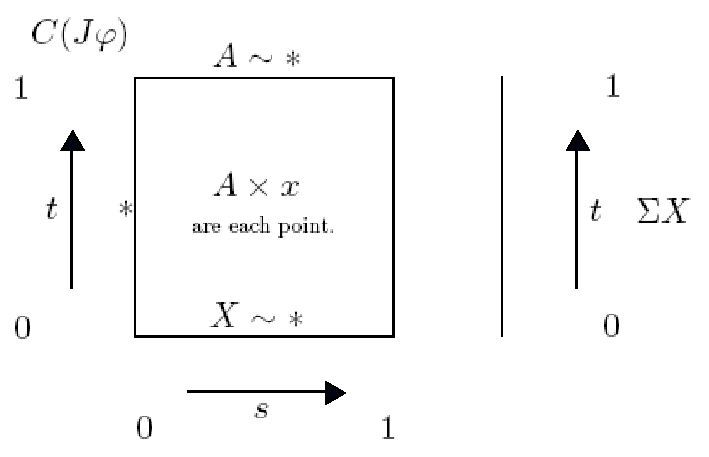
\includegraphics[width=0.3\textwidth]{figures/figure32.pdf}
\caption{\small Diagram of $CJ\varphi$.}
\end{figure}
\begin{figure}[ht!]
\centering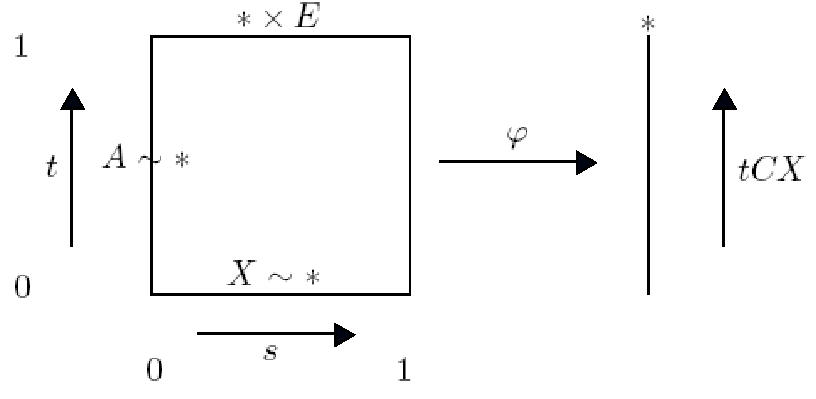
\includegraphics[width=0.3\textwidth]{figures/figure33.pdf}
\caption{\small Diagram of $T\varphi$.}
\end{figure}

So both pictures really are the same; they both look like a triangle.
\begin{figure}[ht!]
\centering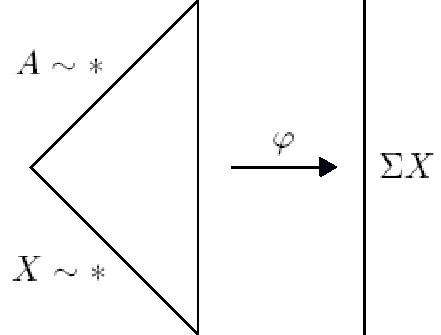
\includegraphics[width=0.2\textwidth]{figures/figure34.pdf}
\caption{\small Triangle!}
\end{figure}
And homeomorphisms with this triangle for the two spaces above are given by
\begin{align*}
f(s, a, t, x) & = \left( \frac{s - st}{1 - st}, a, st, x \right), \\
g(s, a, t, x) & = \left( s + t - st, a, \frac{t}{s + t - st}, x \right).
\end{align*}
\end{proof}

Remember how we got here: we were studying the EHP spectral sequence.  This spectral sequence has as its columns the homotopy groups of odd spheres and converged to $\pi_* QS^0 = \pi_*^S S^p$; moreover we had arranged it so that beneath a line of slope $2$, the entries in each column were the stable homotopy of spheres: \todo{INKSCAPE}  This feature suggested the question: is there a spectral sequence whose columns are the stable homotopy of spheres and a map of spectral sequences from the EHPSS to this SS such that the map is an isomorphism below the celebrated line of slope 2?

On Friday we constructed a candidate, an Atiyah-Hirzebruch spectral sequence for the attaching maps on $\RP^\infty$: $\widetilde H^*(\RP^\infty_+; \pi_*^S)$ which we hope converges to $\pi_*^S \RP^\infty_+$, whose $E^1$-term is \todo{INKSCAPE}

Sure enough, there is a spectral sequence map between these two spectral sequences which is an isomorphism below the line at $E^1$.  To see this, remember the EHP sequence: $\Loops^{n-1} S^{n-1} \to \Loops^n S^n \to \Loops^n S^{2n-1}$.  Here we looped it $(n-1)$ times as this is the form in which it went into the EHPSS.  This is a fibration, strictly if $n$ is even or localized at $2$ if $n$ is odd.  Linking these together and applying $\pi_*$ gave us the EHPSS.  On the other hand, the AHSS from Friday came from taking the cofibration sequence \[\RP^{n-2}_+ \to \RP^{n-1}_+ \to S^{n-1}_+\] and applying $\pi_*^S = \pi_* Q$.  (Recall $QX = \bigcup_k \Loops^k \Suspend^k X$.)  The sequence \[Q\RP^{n-2}_+ \to Q\RP^{n-1}_+ \to QS^{n-1}_+\] is a fibration, since $\pi_*^S$ is a homology theory and hence exact on \[\RP^{n-2}_+ \to \RP^{n-1}_+ \to S^{n-1}_+.\]  Next, note that we have \[S^{n-1}_+ \xrightarrow{e^n} \Loops^n S^{2n-1}_+ \xrightarrow{e^{\infty-n}} QS^{n-1}_+,\] and $e^{\infty-n}$ is an isomorphism on $\pi_*$ for $* < n$.

\begin{thm}
There are maps $s_n$ (``Snaith maps'' or ``Hopf-James'' maps\footnote{Oh dear.}) with
\begin{ctikzcd}
\Loops^{n-1} S^{n-1} \dar["s_{n-1}"]\rar & \Loops^n S^n \dar["s_{n}"]\rar & \Loops^n S^{2n-1} \dar["e^{\infty-n}"]\\
Q \RP^{n-2}_+ \rar & Q\RP^{n-1}_+ \rar & QS^{n-1}_+.
\end{ctikzcd}
\end{thm}
So this theorem does it.  This is a wonderful theorem; we'll try to prove it.  It was probably first proved by Nick Kuhn, although the maps are constructed by Smith.  Before we go on though, we should note two corollaries which answer an old question we've been trying to answer for a long time now.
\begin{cor}
In the portion of these sequences
\begin{cjointikzcd}[intertext,diagram sep=large]
\diagram
    \pi_{n-1} \Loops^n S^{2n-1} \dar["e^{\infty-n}"]\rar["p"] & \pi_{n-2} \Loops^{n-1} S^{n-1}\dar["s_{n+1}"] \\
    \pi_{n-1}^S S^{n-1} \rar & \pi_{n-2}^S \RP^{n-2}_+
%
\diagram \intertext{we have}
%
\diagram
    \iota \dar[mapsto] \rar[mapsto,"p"] & w_{n-1} \dar[mapsto]\\
    \iota \rar[mapsto] & \pi,
\end{cjointikzcd}
where $\pi$ is the stable homotopy class of the attaching map for the top cell in $\RP^{n-1}$ as before.
\end{cor}
\begin{proof}
The top row we've known for a while; the left leg is obvious.  The bottom row is almost as obvious; we'll have the Barratt-Puppe sequence
\begin{ctikzcd}
S^{n-1} \rar & \RP^{n-2} \rar &  \RP^{n-1} = C\pi \rar &  S^{n-1} \rar["\Suspend\pi"] & \RP^{n-2}
\end{ctikzcd}
in which the middle two maps are the cofibration on which the maps above were defined.
\end{proof}
Well, we have already deduced what happens to $\pi$ in the AHSS: the differentials on the various $\pi$ hit elements in the image of the $J$-homomorphism.
\begin{thm}
So $w_{n-1}$ desuspends to an element in $\pi_{2n-\rho(n)-2} S^{n-\rho(n)}$ and no further.
\end{thm}

% >>>
\fi
\BoxedNote{}







\section{The space of little cubes} % <<<
\label{TheSpaceOfLittleCubes}
\ifx\OutputTheSpaceOfLittleCubes\undefined\else
Today we'll examine where the Snaith maps come from, but you're going to have to believe some things.  Some references for this include May's book~\cite{May}, Cohen's paper~\cite{Cohen}, and Kuhn's paper~\cite{Kuhn}.  Remember, we're trying to construct maps
\begin{ctikzcd}
\Loops^n S^0 \rar["s_n"] & Q\RP^{n-1}.
\end{ctikzcd}
Because constructing maps out of loop spaces is hard, we'd like a tractable model for $\Loops^n S^n$.  Fortunately, there are some hints as to how to proceed.

\begin{figure}[ht!]
\centering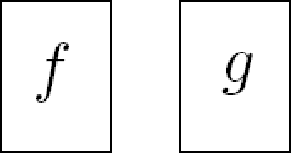
\includegraphics[width=0.2\textwidth]{figures/figure35-1.pdf}\;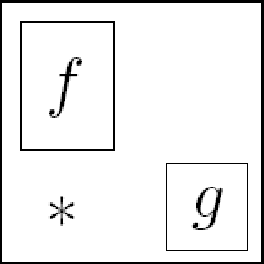
\includegraphics[width=0.2\textwidth]{figures/figure35-2.pdf}\;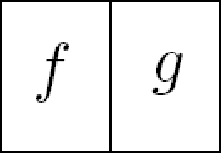
\includegraphics[width=0.2\textwidth]{figures/figure35-3.pdf}\;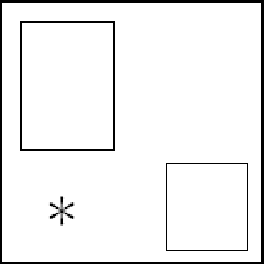
\includegraphics[width=0.2\textwidth]{figures/figure35-4.pdf}
\caption{\small $\Loops^2 X$ and the little cubes operad.}
\end{figure}
First, we do have the map $\Loops^2 X \times \Loops^2 X \to \Loops^2 X$ giving the $H$-space structure; if we represent $f \in \Loops^2 X$ and $g \in \Loops^2 X$ by the leftmost pair of boxes where the edges go to the basepoint, then their product could be represented by the second leftmost diagram, for example.  Of course, the usual representative is the second rightmost, but you have to fiddle with this any way, for example to show the product is associative or commutative up to homotopy.\todo{These figures could use repair.}  This motivates us to study spaces of rectangles.  For example, the rightmost diagram is a point in $C_2(2)$ (two rectanges in $I^2$); in general, the space $C_k(n)$ will be
\[
C_k(n) = \{ \hbox{space of $k$ disjoint parallel $n$-rectangles in $I^n$} \}
,\]
so what you're really describing is the space of embeddings $\coprod_k I^n \into I^n$.  This is called the space of ``little cubes.''  This space parameterizes the multiplication in $\Loops^n X$; namely for each $k$ we have a map $C_k(n) \times (\Loops^n X)^k \to \Loops^n X$. These piece together to give $\coprod_{k \ge 1} C_k(n) \times (\Loops^n X)^k \to \Loops^n X$.

To model the multiplicative structure you have to make some identifications:
\begin{enumerate}
\item The constant loop obliterates a cube; e.g.:
\begin{center}
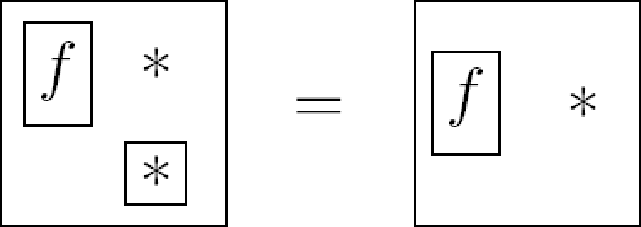
\includegraphics[width=0.2\textwidth]{figures/figure36.pdf}
\end{center}
\item The symmetric group $\Sigma_k$ acts diagonally on $C_k(n) \times (\Loops^n X)^k$, and the map is equivariant with respect to this action.
\end{enumerate}

Now if $X = \Suspend^n A$ then we have the map $\alpha: A \to \Loops^n \Sigma^n A=\Loops^n X$, and get
\begin{ctikzcd}[row sep=small]
\coprod_{k \ge 1} C_k(n) \times_{\Sigma_k} (\Loops^n X)^k / \sim \rar & \Loops^n \Suspend^n A \\
\coprod_{k \ge 1} C_k(n) \times_{\Sigma_k} A^k / \sim \uar,
\end{ctikzcd}
with the bottom $\sim$ meaning the identification in 1) above, which we won't mark down from now on.

\begin{thm}[May]
If $A$ is path-connected, this composite is a weak equivalence.
\end{thm}
This is the basic theorem in the theory of iterated loop spaces.  Note that it bears some resemblance to James' theorem.

Now you can replace each cube with its center; obviously the size of the cube doesn't affect homotopy properties.  So we get a $\Sigma_k$-equivariant equivalence
\begin{ctikzcd}
C_k(n) \rar["\simeq", "\Sigma_k"'] & F_k \Rbb^n,
\end{ctikzcd}
where $F_k(W)$ is defined to be the space of $k$-tuples in $W$ with no repeated elements.  So we have
\begin{ctikzcd}
\coprod_{k \ge 1} F_k \Rbb^n \times_{\Sigma_k} A^k / \sim & \lar["\simeq"'] \coprod_{k \ge 1} C_k(n) \times_{\Sigma_k} A^k / \sim \rar & \Loops^n \Suspend^n A.
\end{ctikzcd}
What's going on?  We're choosing $k$ many points, and rather than ordering we're labeling them with a point of $A$.  It can be constructive to think of the label as a sort of ``charge''; if the charge is zero (i.e., the point is labeled by the basepoint), we're ignoring it.  Call this space $C(\Rbb^n, A)$, following Fred Cohen's notation.

This is a pretty simple model, and we ought to be able to understand it.  Let's relate it to the James construction: so let $n = 1$.  In this case, $F_k(\Rbb^1)$ is equivalent $\Sigma_k$-equivariantly to $\{t_1 < \cdots < t_k\} \times \Sigma_k$.  In this case the God-given ordering on $\Rbb^1$ tells us the unique permutation to bring a collection of poiints into standard order.  So
\begin{ctikzcd}
C(\Rbb, A) \drar["\simeq"']\rar[equal] & \coprod_k \{t_1 < \cdots < t_k\} \times A_k / \sim \dar["\simeq"]\\
 & \coprod A^k / \sim,
\end{ctikzcd}
where $\coprod A^k / \sim$ is the James construction $J(A)$, the ``free monoid'' on $A$.  So $C(\Rbb^n, A)$ really is a generalization of the James construction.

In order to study $C(\Rbb^n, A)$, look at the obvious filtration $F(W, A)_k = \coprod_{j \le k} F_j(W) \times_{\Sigma_j} A / \sim$.  The associated quotient is
\begin{align*}
D_k(W, A) & = F_k / F_{k-1} \\
& = F_k(W) \times_{\Sigma_k} A^k / F_k(W) \times_{\Sigma_k} \{\hbox{fat wedge of} A\} \\
& = F_k(W) \times_{\Sigma_k} A^{\sprod k} / F_k(W) \times_{\Sigma_k} \ptspace.
\end{align*}
Now consider the case $A = S^q$, so that $(S^q)^{\sprod k} =_{\Sigma_k} (\Rbb^k)^q_+$, where the ``${}_+$'' denotes the $1$-point compactification.  Writing $\xi_k$ for the vector bundle $\xi_k = F_k(W) \times_{\Sigma_k} \Rbb^k$ over $B_k(W) = F_k(W) / \Sigma_k$, then $F_k / F_{k-1} = D_k(W, S^q) = T(q\xi_k \downarrow B_k(W))$.  It follows that $C(W, A)$ has a filtration whose successive quotients are Thom spaces.  In the example $W = \Rbb^n$ and $k = 2$, we have
\begin{ctikzcd}[row sep=0pt]
F_2(\Rbb^n) \rar["\cong"',"\Sigma_2"] & \Rbb^n \times (\Rbb^n \setminus \{0\}) \\
(x, y) \rar[mapsto] & \left( \frac{x + y}{2}, \frac{x - y}{2} \right),
\end{ctikzcd}
and $B_2(\Rbb^n) \cong \Rbb^{n+1} \times  \RP^{n-1}$.  We can compute $\xi_2 = 1 + L$ over $\Rbb^{n+1} \times \RP^{n-1}$, and hence \[T \xi_2 = D_2(\Rbb^2, S^q) = T(q(1+K) \downarrow \RP^{n-1}) = \Suspend^q \RP^{n+q-1}_q.\]  This is a good sign: we got a stunted projective space.

Here's another useful example: we claim that the inclusion $F_k(\Rbb^{n-1}) \into F_k(\Rbb^n)$ is null-homotopic.  A basepoint in $F_k(\Rbb^n)$ consists of a choice of $k$ distinct points, and any $k$ points in $\Rbb{n-1}$ can be smoothly moved to the fixed set of points in $\Rbb^n$ (cf., Figure \ref{ContractibilityOfFkRinfty}).
\begin{figure}%used to be [!ht]
\centering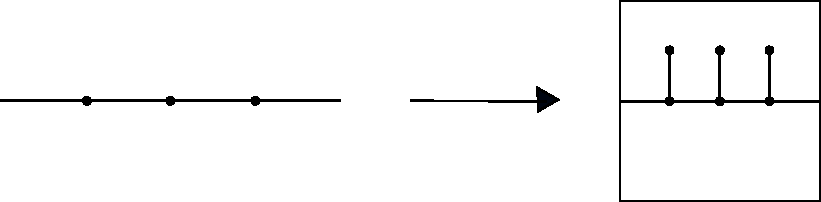
\includegraphics[width=0.35\textwidth]{figures/figure37.pdf}
\caption{\small Contractibility of $F_k \Rbb^\infty$.}\label{ContractibilityOfFkRinfty}
\end{figure}
\noindent This means that $F_k(\Rbb^\infty) = \bigcup_n F_k(\Rbb^n)$ is a contractible space with a free $\Sigma_k$-action, so it's an $E_{\Sigma_k}$ and $F_k(\Rbb^\infty) \downarrow B_k(\Rbb^\infty)$ is a universal $\Sigma_k$-bundle, and
\begin{align*}
Q(A) & = \bigcup_n \Loops^n \Suspend^n A \\
& = \bigcup_n \coprod_{k \ge 1} F_k(\Rbb^n) \times_{\Sigma_k} A^k \\
& = \coprod_{k \ge 1} E_{\Sigma_k} \times_{\Sigma_k} A^k / \sim.
\end{align*}

Let's see now how to use this to produce maps.  We're going to do this in blinding generality; namely, the map $s_k$ will be a map
\[
s_k: C(W, A) \to C(B_k(W), D_k(W, A))
\]
so a point of $C(W, A)$ is a finite subset $S \subset W$ and an assignment $f: S \to A$.  We have to take this to a finite subset $s_k S$ of points of $B_k(W)$.  The points of $B_k(W)$ are $k$-tuples in $W$, so we take for $s_k S$ the set $\{T \subseteq S : |T| = k\}$.  In addition to $s_k S$ we need an assignment $s_k f$ of points in $s_k S$ to charges in $D_k(W, A)$.  But a charge in $D_k(W, A)$ is an assignment of charges in $A$ to a $k$-element subset of $W$.  So for $T \in s_k S$, we define $s_kf(T) = f|_T$.

Now take the case $W = \Rbb^n$ and $A$ path-connected.  Then
\begin{ctikzcd}
C(W, A) \rar["\simeq","\mathrm{weak}"'] & \Loops^n \Suspend^n A \dar[into]\rar{s_k} & C(B_k(\Rbb^n), D_k(\Rbb^n, A)) \\
& C(\Rbb^N, D_k(\Rbb^n, A)) \dar[into] \\
& \Loops^N \Suspend^N D_k(\Rbb^n, A).
\end{ctikzcd}
Now when $A = S^1$ (you'd like to take $A=S^0$ but it's not connected), you get
\[
s_2: \Loops^n S^{n+1} \to \Loops^N \Suspend^N(\Suspend \RP^n)
.\]
So, looping once,
\begin{ctikzcd}
\Loops^{n+1} S^{n+1} \rar["s"] & \Loops^{N+1}\Suspend^{N+1} \RP^n \rar & Q \RP^n.
\end{ctikzcd}
There's lots of work still to be done: you have to check the compatibility of the maps and so forth.  But the model's so simple it's not hard to believe that it works.  For more information, see Kuhn's paper~\cite{Kuhn}.

% >>>
\fi
\BoxedNote{}
